\documentclass[twoside,11pt]{report}
% ============================================================ EX-TEST
\usepackage[utf8]{vietnam}
\usepackage{ex_test}
%\usepackage[solcolor]{ex_test} % dethi, color, loigiai, solcolor, book
\renewtheorem{ex}{\color{blue!90!black} Câu}
\usepackage{amsmath,amssymb,tikz,mathrsfs,tkz-tab}
\usepackage{fontawesome}
\usepackage[many]{tcolorbox}
\usetikzlibrary{calc}
\usepackage{geometry}
\renewcommand{\baselinestretch}{1.5}
\usepackage[locale=DE]{siunitx} % cách viết số đo có đơn vị theo chuẩn DE (gần giống VN) 
\usepackage{setspace} % hỗ trợ định dạng khoảng cách văn bản.
\usepackage[newparttoc]{titlesec}	% định dạng tiêu đề cho các section
\usepackage{currfile}
\usepackage[version=3]{mhchem} % công thức và phương trình hóa học 
\usepackage{tikz} % gói TikZ vẽ hình 
\usetikzlibrary{decorations.shapes,shapes.geometric,calc,positioning}
\usepackage{pgf} % hỗ trợ phép tính toán học và vẽ hình	
\usetikzlibrary{shapes.geometric, arrows}
\usepackage{pgfplots}
\renewcommand{\baselinestretch}{1.2}
\usepackage{tabularx}
\usepackage{makecell}
\usepackage{titlesec}
\usepackage{titletoc}
\usepackage{colortbl}
\usepackage{capt-of}
% lệnh siunit 
\newcommand{\xsi}[2]{\SI[parse-numbers=false]{#1}{#2}}
\newcommand{\outfooter}{
	\color{purple}\bfseries	GV: Lương Hoàng Sang
}
\newcommand{\outheader}{
	\color{purple}\bfseries	Trường THCS - THPT Nguyễn Khuyến
}
\newcommand{\namhoc}{
	\color{purple}\bfseries	Năm học: 2024 - 2025
}
\def\monhoc{\bfseries Vật lí 10}%{\bfseries Kế hoạch bài dạy vật lí 10}
\graphicspath{{figs/}{extra/}} % các thư mục chứa hình ảnh 

% ========== PAPER FORMAT ====================
% --- paper size 
\geometry{
	a4paper	% khổ giấy A4
	,total={180mm,260mm} % kích thước văn bản A4 170mmx247mm
	,left=15mm % canh lề trái
	,top=20mm % canh lề trên
	,footskip=1.0cm % khoảng cách từ văn bản đến footer
}
% --- line spacing -- choose 1 in 2 choices 
\onehalfspacing			% cách dòng đơn
%\doublespacing			% cách dòng đôi  
% ----- định dạng Header và footer
% --- 
\newlength\sectitleindent
\setlength\sectitleindent{0.5cm}
\newlength\subsectitleindent
\setlength\subsectitleindent{1cm}
% --- trang văn bản thông thường  
\pagestyle{fancy} 
\fancyhf{}
\renewcommand{\headrulewidth}
{1pt} % độ dày đường kẻ ở header 
\newcommand*\cirpage[1] % tạo hình tròn quanh số trang 
{\tikz[baseline=(char.base)]
	{
		\node[
		shape=circle
		,draw=black
		,fill=gray!0
		,inner sep=2pt
		]
		(char)
		{#1};
	}
}
\fancyhead[LO,RE] % footer - lề trong 
{	
	\small \outheader \hfill \namhoc% tên tài liệu lấy từ phần khai báo đầu file 
}  
\fancyfoot[LO,RE] % footer - lề trong 
{	
	\small \outfooter % tên tài liệu lấy từ phần khai báo đầu file 
}  
\fancyfoot[CO,CE] % footer - giữa trang 
{
	\small \cirpage{\thepage}
} 
\fancyfoot[LE] % footer - lề ngoài 
{
	\hspace{-\sectitleindent}
	\vspace*{-11pt}
	{\color{purple} \monhoc}
}
\fancyfoot[RO] % footer - lề ngoài 
{
	\hspace{-\sectitleindent}
	\vspace*{-11pt}
	{\color{purple} \monhoc}\hspace*{-5pt}
}
% --- trang Part và Chapter title 
\fancypagestyle{plain} % mặc định của trang Part và Chapter title 
{
	\fancyfoot[LO,RE]
	{
		\hspace{-\sectitleindent}\small \outfooter
	}
	\fancyfoot[CO,CE]
	{
		\small \cirpage{\thepage}
	} % footer - giữa trang chẵn và lẻ 
	\fancyfoot[LE]
	{
		\hspace{-\sectitleindent}
		\vspace*{-11pt}
		\hspace*{-1.1pt}{\color{purple}\monhoc}
	}
	\fancyfoot[RO]
	{
		\hspace{-\sectitleindent}
		\vspace*{-11pt}
		{\color{purple}\monhoc}\hspace*{-5pt}
	}
} % giống với trang thường 
% ký hiệu từ font Boondox 
\DeclareFontFamily{U}{BOONDOX-cal}{\skewchar\font=45 }
\DeclareFontShape{U}{BOONDOX-cal}{m}{n}{
	<-> s*[1.05] BOONDOX-r-cal}{}
\DeclareFontShape{U}{BOONDOX-cal}{b}{n}{
	<-> s*[1.05] BOONDOX-b-cal}{}
\DeclareMathAlphabet{\bdx}{U}{BOONDOX-cal}{m}{n}
\SetMathAlphabet{\bdx}{bold}{U}{BOONDOX-cal}{b}{n}
\DeclareMathAlphabet{\bbdx}{U}{BOONDOX-cal}{b}{n}
\newcommand{\calE}{\bdx{E}}
\newcommand{\calP}{\bdx{P}}
\newcolumntype{C}[1]{>{\centering\arraybackslash}p{#1}}
\newcolumntype{M}[1]{>{\centering\arraybackslash}m{#1}}
\newcolumntype{L}[1]{>{\raggedright\arraybackslash}p{#1}}
\newcommand{\hoac}[1]{ %hệ hoặc
	\left[\begin{aligned}#1\end{aligned}\right.}
\newcommand{\heva}[1]{ %hệ và
	\left\{\begin{aligned}#1\end{aligned}\right.}

\begin{document}
	\renewcommand{\thesection}{\Roman{section}}
	\titleformat{\section}
	{\normalfont\bfseries}{PHẦN~\thesection.}{0.4em}{}
	\newcolumntype{C}[1]{>{\centering\arraybackslash}p{#1}}
	\newcolumntype{M}[1]{>{\centering\arraybackslash}m{#1}}
	\newcolumntype{L}[1]{>{\raggedright\arraybackslash}p{#1}}
	\renewcommand{\theadfont}
	{
		\normalfont\bfseries
	}
%	\begin{tabular}{C{6cm}C{11cm}}
%		\textbf{TRUNG TÂM MANABIE}& \textbf{ĐỀ KIỂM TRA ĐẦU CHƯƠNG LỚP 12} \\
%		\textbf{ĐỀ PH12D02}& \textbf{Môn: VẬT LÝ}\\
%		\textit{(Đề có 04 trang)}& \textit{Thời gian làm bài: 45 phút, không kể thời gian phát đề}
%		
%		\noindent\rule{4cm}{0.8pt} \\
%	\end{tabular}
%\newcommand{\hoac}[1]{ %hệ hoặc
%	\left[\begin{aligned}#1\end{aligned}\right.}
%\newcommand{\heva}[1]{ %hệ và
%	\left\{\begin{aligned}#1\end{aligned}\right.}
% ====================================================== input data BT1+2
%\setcounter{section}{0}
\section{Câu trắc nghiệm nhiều phương án lựa chọn}
\textit{Thí sinh trả lời từ câu 1 đến câu 18. Mỗi câu hỏi thí sinh chọn một phương án}
\setcounter{ex}{0}
\Opensolutionfile{ans}[ans/G12C1TN]
%-------------------------
\begin{ex}
	"Độ không tuyệt đối" là nhiệt độ ứng với
	\choice
	{\True $\SI{0}{\kelvin}$}
	{$\SI{0}{\celsius}$}
	{$\SI{273}{\celsius}$}
	{$\SI{273}{\kelvin}$}
	\loigiai{
	}
	\end{ex}
% ===================================================================
\begin{ex}
\immini{
	Hình bên mô tả chuyển động phân tử ở các thể khác nhau. Hình cầu là phân tử, mũi tên là hướng chuyển động của phân tử. Hình mô tả chuyển động phân tử tương ứng với thể rắn, thể lỏng và thể khí lần lượt là
}
{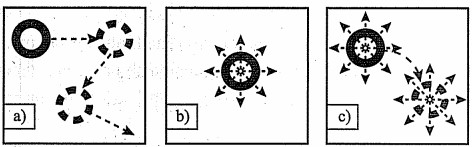
\includegraphics[scale=0.7]{figs/G12-C1-4}
}
\choice
{a), b), c)}
{\True b), c), a)}
{c), b), a)}
{b), a), c)}
	\loigiai{}
\end{ex}
% ===================================================================
\begin{ex}
	Hãy tìm ý \textbf{không đúng} với mô hình động học phân tử.
	\choice
	{Các chất được cấu tạo từ các hạt riêng biệt là phân tử}
	{Các phân tử chuyển động không ngừng}
	{\True Tốc độ chuyển động của các phân tử cấu tạo nên vật càng lớn thì thể tích của vật càng lớn}
	{Giữa các phân tử có lực tương tác gọi là lực liên kết phân tử}
	\loigiai{}
\end{ex}
% ===================================================================
\begin{ex}
	Hãy chọn phương án \textbf{sai} trong các câu sau: Cùng một khối lượng của một chất nhưng khi ở các thể tích khác nhau thì sẽ khác nhau
	\choice
	{thể tích}
	{khối lượng riêng}
	{\True kích thước của các nguyên tử}
	{trật tự của các nguyên tử}
	\loigiai{}
\end{ex}


% ===================================================================
\begin{ex}
Vật ở thể lỏng có	
	\choice
	{thể tích và hình dạng riêng, khó nén}
	{thể tích và hình dạng riêng, dễ nén}
	{\True thể tích riêng nhưng không có hình dạng riêng, khó nén}
	{thể tích riêng nhưng không có hình dạng riêng, dễ nén}
	\loigiai{}
\end{ex}

% ===================================================================
\begin{ex}
	Khi nói đến nhiệt độ của một vật ta thường nghĩ đến cảm giác "nóng" và "lạnh" của vật nhưng đó chỉ là tương đối vì cảm giác mang tính chủ quan. Cảm giác nóng, lạnh mà chúng ta cảm nhận được khi tiếp xúc với vật liên quan đến
	\choice
	{\True năng lượng nhiệt của các phân tử}
	{khối lượng của vật}
	{trọng lượng riêng của vật}
	{động năng chuyển động của vật}
	\loigiai{}
\end{ex}
% ===================================================================
\begin{ex}
	Nội năng của một vật là
	\choice
	{tổng động năng và thế năng của vật}
	{\True tổng động năng và thế năng của các phân tử cấu tạo nên vật}
	{tổng nhiệt lượng và cơ năng mà vật nhận được trong quá trình truyền nhiệt và thực hiện công}
	{nhiệt lượng vật nhận được trong quá trình truyền nhiệt}
	\loigiai{}
\end{ex}
% ===================================================================
\begin{ex}
	Phát biểu nào sau đây là \textbf{đúng}?
	\choice
	{Nội năng của một hệ nhất định phải có thế năng tương tác giữa các hạt cấu tạo nên vật}
	{Nhiệt lượng truyền cho hệ chỉ làm tăng động năng của chuyển động nhiệt của các hạt cấu tạo nên hệ}
	{\True Công mà hệ nhận được có thể làm thay đổi cả tổng động năng chuyển động nhiệt của các hạt cấu tạo nên hệ và thế năng tương tác giữa chúng}
	{Nói chung, nội năng là hàm của nhiệt độ và thể tích, nên nếu thể tích của hệ đã thay đổi thì nội năng của hệ phải thay đổi}
	\loigiai{}
\end{ex}

% ===================================================================
\begin{ex}
	Nhiệt lượng được truyền vào hỗn hợp nước đá để làm tan chảy một phần nước đá. Trong quá trình này, hỗn hợp nước đá
	\choice
	{thực hiện công}
	{có nhiệt độ tăng lên}
	{\True có nội năng tăng lên}
	{thực hiện công, có nhiệt độ tăng và nội năng cũng tăng}
	\loigiai{}
\end{ex}

% ===================================================================
\begin{ex}
	\immini{Hình bên là đồ thị phác hoạ sự thay đổi nhiệt độ theo thời gian trong quá trình chuyển thể từ rắn sang lỏng của chất rắn kết tinh và của chất rắn vô định hình tương ứng lần lượt là
	\choice
	{\True đường (3) và đường (2)}
	{đường (1) và đường (2)}
	{đường (2) và đường (3)}
	{đường (3) và đường (1)}
}{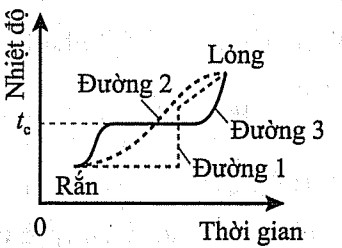
\includegraphics[scale=0.6]{figs/G12-C1-1}}
\loigiai{
\begin{itemize}
	\item Khi nung nóng liên tục một vật rắn kết tinh, nhiệt độ của vật rắn tăng dần. Khi nhiệt độ đạt đến nhiệt độ nóng chảy thì vật bắt đầu chuyển sang thể lỏng và trong suốt quá trình này nhiệt độ của vật không thay đổi. Khi toàn bộ vật rắn đã chuyển sang thể lỏng, nếu tiếp tục cung cấp nhiệt lượng thì nhiệt độ của vật sẽ tiếp tục tăng (đường 3).
	\item Khi nung nóng liên tục vật rắn vô định hình, vật rắn mềm đi và chuyển dần sang thể lỏng một cách liên tục. Trong quá trình này, nhiệt độ của vật tăng lên liên tục. Do đó, vật rắn vô định hình không có nhiệt độ nóng chảy xác định (đường 2).
\end{itemize}
}
	
\end{ex}
% ===================================================================
\begin{ex}
	Gọi $x$, $y$ và $z$ lần lượt là khoảng cách trung bình giữa các phân tử của một chất ở thể rắn, lỏng và khí. Hệ thức đúng là
	\choice
	{$z<y<x$}
	{$x<z<y$}
	{$y<x<z$}
	{\True $x<y<z$}
	\loigiai{}
\end{ex}
% ===================================================================
\begin{ex}
	Một quả bóng có khối lượng $\SI{100}{\gram}$ rơi từ độ cao $\SI{10}{\meter}$ xuống sân và nảy lên được $\SI{7}{\meter}$. Sở dĩ bóng không nảy lên được tới độ cao ban đầu là vì một phần cơ năng của quả bóng đã chuyển hoá thành nội năng của
	\choice
	{chỉ quả bóng và sân}
	{chỉ quả bóng và không khí}
	{chỉ mỗi sân và không khí}
	{\True quả bóng, mặt sân và không khí}
	\loigiai{}
\end{ex}

% ===================================================================
\begin{ex}
	Nếu thực hiện công $\SI{100}{\joule}$ để nén khí trong một xilanh thì khí truyền ra môi trường xung quanh nhiệt lượng $\SI{30}{\joule}$. Xác định độ thay đổi nội năng của khí trong cylanh.
	\choice
	{$\SI{50}{\joule}$}
	{$\SI{60}{\joule}$}
	{$\SI{30}{\joule}$}
	{\True $\SI{70}{\joule}$}
	\loigiai{Hệ nhận công và nhả nhiệt nên: $A=\SI{100}{\joule}$ và $Q=\SI{-30}{\joule}$.\\
		Độ biến thiên nội năng của khí trong xilanh:
		$$\Delta U=A+Q=\SI{70}{\joule}.$$}
\end{ex}
% ===================================================================
\begin{ex}
	Một vật được làm lạnh từ $\SI{25}{\celsius}$ xuống $\SI{5}{\celsius}$. Nhiệt độ của vật theo thang Kelvin giảm đi bao nhiêu Kelvin?
	\choice
	{$\SI{15}{\kelvin}$}
	{\True $\SI{20}{\kelvin}$}
	{$\SI{11}{\kelvin}$}
	{$\SI{18}{\kelvin}$}
	\loigiai{$$\Delta T=\Delta t=\SI{-20}{\kelvin}.$$}
\end{ex}
% ===================================================================
\begin{ex}
Một bình đựng nước ở $\SI{0.00}{\celsius}$. Người ta làm nước trong bình động đặc lại bằng cách hút không khí và hơi nước trong bình ra ngoài. Lấy nhiệt nóng chảy riêng của nước là $\SI{3.3E5}{\joule/\kilogram}$ và nhiệt hoá hơi riêng của nước là $\SI{2.48E6}{\joule/\kilogram}$. Bỏ qua sự trao đổi nhiệt với môi trường bên ngoài. Tỉ số giữa khối lượng nước bị hoá hơi và khối lượng nước ở trong bình lúc đầu là
	\choice
	{\True 0,12}
	{0,84}
	{0,16}
	{0,007}
	\loigiai{Gọi $m$ và $m'$ lần lượt là khối lượng nước ban đầu và khối lượng nước bị hoá hơi. Nhiệt lượng làm hoá hơi hoàn toàn khối lượng nước $m'$ bằng nhiệt lượng làm đông đặc hoàn toàn khối lượng nước $\left(m-m'\right)$.\\
	Ta có:
$$Q_\text{đ}=Q_h\Rightarrow \left(m-m'\right)\lambda=m'L\Rightarrow\dfrac{m'}{m}=\dfrac{\lambda}{\lambda+L}=0,12.$$}
\end{ex}
% ===================================================================
\begin{ex}
	Một học sinh, sau khi biết đến thí nghiệm nổi tiếng của Joule, đã phát triển một thiết bị đạp xe cố định (tập gym), có thể chuyển đổi toàn bộ năng lượng tiêu hao thành nhiệt để làm ấm nước. Cần bao nhiêu cơ năng để tăng nhiệt độ của $\SI{300}{\gram}$ nước $\SI{20}{\celsius}$ đến $\SI{95}{\celsius}$? Biết nhiệt dung riêng của nước là $\SI{4200}{\joule/\left(\kilogram\cdot\kelvin\right)}$.
	\choice
	{\True $\SI{94500}{\joule}$}
	{$\SI{22000}{\joule}$}
	{$\SI{5400}{\joule}$}
	{$\SI{14}{\joule}$}
	\loigiai{
$$Q=mc\Delta T=\SI{94500}{\joule}.$$
}
\end{ex}

% ===================================================================
\begin{ex}
	\immini{Một học sinh dùng một sợi dây buộc vào một vật có khối lượng $\SI{5.0E2}{\kilogram}$ đang rơi qua ròng rọc vào trục bánh guồng. Học sinh này đặt hệ thống vào một bể chứa $\SI{25.0}{\kilogram}$ nước cách nhiệt tốt. Khi vật rơi xuống sẽ làm cho bánh guồng quay và khuấy động nước. Nếu vật rơi một khoảng cách thẳng đứng $\SI{1.00E2}{\meter}$ với vận tốc không đổi thì nhiệt độ của nước tăng bao nhiêu độ? Biết nhiệt dung riêng của nước là $\SI{4.20}{\kilo\joule/\left(\kilogram\cdot\kelvin\right)}$, $g=\SI{9.81}{\meter/\second^2}$.
	\choice
	{$\SI{15}{\kelvin}$}
	{\True $\SI{4.7}{\kelvin}$}
	{$\SI{6.1}{\kelvin}$}
	{$\SI{18}{\kelvin}$}
}
{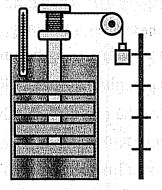
\includegraphics[scale=0.8]{figs/G12-C1-2}}
	\loigiai{Vì vật rơi với vận tốc không đổi nên độ giảm thế năng của nó dùng để làm tăng nhiệt độ cho bình nước.
	$$mgh=m'c\Delta T\Rightarrow \Delta T=\dfrac{mgh}{m'c}=\SI{4.7}{\kilogram}.$$}
\end{ex}
% ===================================================================
\begin{ex}
Một bình cách nhiệt được ngăn làm hai phần bằng một vách ngăn cách nhiệt. Hai phần bình chứa 2 chất lỏng có nhiệt dung riêng $c_1$, $c_2$ và nhiệt độ $t_1$, $t_2$ khác nhau. Bỏ vách ngăn, hai khối chất lỏng không tác dụng hoá học với nhau, nhiệt độ của chất lỏng trong bình sau khi cân bằng nhiệt là $t$. Biết rằng $t_1-t=\dfrac{1}{2}\left(t_1-t_2\right)$. Tỉ số $m_1/m_2$ là	
	\choice
	{$\dfrac{c_1}{c_2}$}
	{\True $\dfrac{c_2}{c_1}$}
	{$\sqrt{\dfrac{c_1}{c_2}}$}
	{$\sqrt{\dfrac{c_2}{c_1}}$}
	\loigiai{
Phương trình cân bằng nhiệt:
\begin{equation}
	m_1c_1\left(t_1-t\right)+m_2c_2\left(t_2-t\right)=0
	\label{eq:C1-5}
\end{equation}	
Theo đề bài, ta có:
$$t_1-t=\dfrac{1}{2}\left(t_1-t_2\right)$$
\begin{equation}
	\Rightarrow t_2-t=t-t_1
	\label{eq:C1-6}
\end{equation}
Thay (\ref{eq:C1-6}) vào (\ref{eq:C1-5}), ta được:
$$m_1c_1\left(t_1-t\right)=m_2c_2\left(t_1-t\right)\Rightarrow \dfrac{m_1}{m_2}=\dfrac{c_2}{c_1}.$$
}
\end{ex}


%-------------------------
\Closesolutionfile{ans}


\section{Câu trắc nghiệm đúng/sai} 
\textit{Thí sinh trả lời từ câu 1 đến câu 4. Trong mỗi ý \textbf{a)}, \textbf{b)}, \textbf{c)}, \textbf{d)} ở mỗi câu, thí sinh chọn đúng hoặc sai}
\setcounter{ex}{0}
\Opensolutionfile{ans}[ans/G12C1TF]
\begin{ex}
	Trong các phát biểu sau đây về sự bay hơi và sự sôi của chất lỏng, phát biểu nào đúng, phát biểu nào sai?
	\choiceTF[t]
	{\True Sự bay hơi là sự hoá hơi xảy ra ở mặt thoáng của khối chất lỏng}
	{\True Sự hoá hơi xảy ra ở cả mặt thoáng và trong lòng của khối chất lỏng khi chất lỏng sôi}
	{Sự bay hơi diễn ra chỉ ở một số nhiệt độ nhất định}
	{\True Sự sôi diễn ra ở nhiệt độ sôi}
	\loigiai{\begin{itemize}
			\item Sự hoá hơi là quá trình chuyển thể từ thể lỏng song thể khí. \item Sự hoá hơi thể hiện qua hai hình thức: sự bay hơi và sự sôi.
			\item Sự sôi xảy ra bên trong và trên bề mặt chất lỏng và chỉ xảy ra ở nhiệt độ sôi.
		\end{itemize}
	}
\end{ex}
% ===============================
\begin{ex}
Hình bên là "giản đồ chuyển thể nhiệt độ/áp suất của nước được đơn giản hoá". Trong các phát biểu sau đây, phát biểu nào đúng, phát biểu nào sai?
\begin{center}
	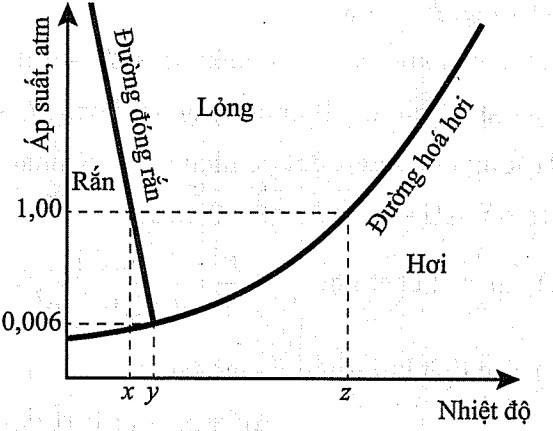
\includegraphics[scale=0.6]{figs/G12-C1-3}
\end{center}
\choiceTF[t]
{\True Thang nhiệt độ Celsius có nhiệt độ dùng làm mốc là nhiệt độ $x$ và nhiệt độ $z$}
{\True Thang nhiệt độ Kelvin có nhiệt độ dùng làm mốc là nhiệt độ thấp nhất mà các vật có thể đạt được (nhiệt độ không tuyệt đối) và nhiệt độ $y$}
{\True Ở nhiệt độ không tuyệt đối, tất cả các chất đều có động năng chuyển động nhiệt của các phân tử bằng không và thế năng của chúng là tối thiểu}
{Hiện nay, các nhà khoa học đã hạ thấp nhiệt độ đến $\SI{0}{\kelvin}$}	


	
	\loigiai{Thang nhiệt độ Celsius có nhiệt độ dùng làm mốc là nhiệt độ tan chảy của nước tinh khiết khi đóng băng và nhiệt độ sôi của nước tinh khiết ở áp suất tiêu chuẩn.\\
	Thang nhiệt độ Kelvin có nhiệt độ dùng làm mốc là nhiệt độ thấp nhất mà các vật có thể đạt được (nhiệt độ không tuyệt đối) và nhiệt độ mà nước tinh khiết có thể tồn tại đồng thời cả ba thể rắn, lỏng và hơi.\\
	Ở nhiệt độ không tuyệt đối, tất cả các chất đều có động năng chuyển động nhiệt của các phân tử bằng không và thế năng của chúng là tối thiểu.\\
	Vật lí học hiện đại chứng tỏ, các hạt không thể đứng yên, điều này có nghĩa chỉ có thể hạ nhiệt độ xuống gần giá trị $\SI{0}{\kelvin}$ nhưng không thể đạt đến giá trị này. Hiện nay, nhiệt độ thấp nhất mà các nhà khoa học có thể tạo ra là $\SI{3.8E-11}{\kelvin}$.
	}
\end{ex}
% ===============================
\begin{ex}
	Nhiệt nóng chảy riêng và nhiệt độ nóng chảy là thông tin, giúp ta có thể
	\choiceTF[t]
	{\True xác định được năng lượng cần cung cấp cho lò nung, thời gian nung}
	{\True thời điểm đổ kim loại nóng chảy vào khuôn, thời điểm lấy sản phẩm ra khỏi khuôn}
	{\True lựa chọn vật liệu chế tạo hợp kim phù hợp với từng yêu cầu sử dụng khác nhau}
	{\True tách các kim loại nguyên chất ra khỏi quặng hỗn hợp}	
	
	\loigiai{}
\end{ex}
% ===============================
\begin{ex}
Một bình đun nước nóng bằng điện có công suất $\SI{9.0}{\kilo\watt}$. Nước được làm nóng khi đi qua buồng đốt của bình. Nước chảy qua buồng đốt với lưu lượng $\SI{5.8E-2}{\kilogram/\second}$. Nhiệt độ của nước khi đi vào buồng đốt là $\SI{15}{\celsius}$. Cho nhiệt dung riêng của nước là $\SI{4200}{\joule/\left(\kilogram\cdot\kelvin\right)}$. Bỏ qua mọi hao phí.
	\choiceTF[t]
	{Nhiệt độ của nước khi ra khỏi buồng đốt là $\SI{50}{\celsius}$}
	{Nếu nhiệt độ của nước khi đi vào buồng đốt tăng gấp đôi thì nhiệt độ nước ra khỏi buồng đốt tăng gấp đôi}
	{\True Nếu công suất điện giảm 2 lần thì nhiệt độ nước ra khỏi buồng đốt là $\SI{33.5}{\celsius}$}
	{\True Để điều chỉnh nhiệt độ của nước ra khỏi buồng đốt, ta có thể thay đổi: công suất điện; lưu lượng nước; nhiệt độ nước đi vào}	

	\loigiai{\begin{itemchoice}
			\itemch Gọi $q$ là lưu lượng nước chảy vào buồng đốt và $\calP$ là công suất buồng đốt.\\
			Nhiệt độ của nước khi ra khỏi buồng đốt:
			$$qtc\left(t_2-t_1\right)=\calP t\Rightarrow t_2=t_1+\dfrac{\calP}{qc}\approx\SI{51.9}{\celsius}.$$
			\itemch Sai vì $t_2=t_1+\dfrac{\calP}{qc}$.
			\itemch Đúng. 
			$$t'_2=t_1+\dfrac{\calP}{2qc}=\SI{33.5}{\celsius}.$$
			\itemch Đúng. $t_2$ phụ thuộc vào $\calP$, $q$ và $t_1$.
			\end{itemchoice}
	}
\end{ex}
\Closesolutionfile{ans}
\section{Câu trắc nghiệm trả lời ngắn} \textit{Thí sinh trả lời từ câu 1 đến câu 6}
\setcounter{ex}{0}
\Opensolutionfile{ans}[ans/G12C1TL]
% ===============================================================
\begin{ex}
	Một người cọ xát một miếng sắt có khối lượng $\SI{0.25}{\kilogram}$ trên một sàn nhà. Sau một thời gian miếng sắt nóng thêm $\SI{12.0}{\celsius}$. Tính công mà người này đã thực hiện \textit{(theo đơn vị $\si{\joule}$, lấy phần nguyên)}. Giả sử rằng $\SI{40}{\percent}$ công đó được dùng làm nóng miếng sắt. Biết nhiệt dung riêng của sắt là $\SI{0.46}{\kilo\joule/\left(\kilogram\cdot\kelvin\right)}$.
	\shortans{$\SI{3450}{}$}
	\loigiai{
		$$0,4A=mc\Delta T\Rightarrow A=\SI{3450}{\joule}.$$
	}
\end{ex}
% ===============================================================
\begin{ex}
	Một viên đạn chì phải có tốc độ tối thiểu là bao nhiêu để khi nó va chạm vào vật cản cứng thì nóng chảy hoàn toàn \textit{(theo đơn vị $\si{\meter/\second}$, lấy phần nguyên)}? Cho rằng $\SI{80.0}{\percent}$ động năng của viên đạn chuyển thành nội năng của nó khi va chạm; Nhiệt độ của viên đạn trước khi và chạm là $\SI{127}{\celsius}$. Cho biết nhiệt dung riêng của chì là $c=\SI{0.130}{\kilo\joule/\left(\kilogram\cdot\kelvin\right)}$; nhiệt độ nóng chảy của chì là $\SI{327}{\celsius}$, nhiệt nóng chảy riêng của chì là $\lambda=\SI{25.0}{\kilo\joule/\kilogram}$.
	\shortans{357}
	\loigiai{
		$$\SI{80}{\percent}\cdot\dfrac{1}{2}mv^2=mc\Delta T+m\lambda\Rightarrow v=\sqrt{\dfrac{2\left(c\Delta T+\lambda\right)}{0,8}}\approx\SI{357}{\meter/\second}.$$
	}
	\end{ex}
	% ===============================================================
\begin{ex}
	Một vật có khối lượng $\SI{1.00}{\kilogram}$ trượt trên một mặt phẳng nghiêng dài $\SI{0.800}{\meter}$ đặt nghiêng $\SI{30.0}{\degree}$. Ở đỉnh của mặt phẳng nghiêng, vận tốc của vật bằng 0; trượt tới chân mặt phẳng nghiêng, tốc độ của vật đạt $\SI{1.10}{\meter/\second}$. Lấy $g=\SI{9.81}{\meter/\second^2}$. Tính nhiệt lượng do vật toả ra do ma sát \textit{(theo đơn vị $\si{\joule}$, lấy đến hai chữ số ở phần thập phân)}.
	\shortans{3,32}
	\loigiai{
		Nhiệt lượng tăng thêm bằng độ lớn công của lực cản và bằng độ giảm cơ năng:
		$$Q=mgh-\dfrac{1}{2}mv^2=mgL\sin\SI{30.0}{\degree}-\dfrac{1}{2}mv^2=\SI{3.32}{\joule}.$$
	}
\end{ex}
	% ===============================================================
\begin{ex}
Ở nhiệt độ $\SI{27}{\celsius}$, các phân tử oxygen chuyển động với tốc độ trung bình khoảng $\SI{500}{\meter/\second}$. Khối lượng của phân tử oxygen là $\SI{53.2E-27}{\kilogram}$. Động năng trung bình của $\SI{E21}{}$ phân tử oxygen bằng bao nhiêu \textit{(viết đáp số 3 kí tự số)}?
	\shortans{6,65}
	\loigiai{
	$$W_\text{đ}=\dfrac{1}{2}Nmv^2=\SI{6.65}{\joule}.$$
	}
\end{ex}
	% ===============================================================
\begin{ex}
Nhiệt lượng kế bằng đồng chứa nước ở $\SI{25}{\celsius}$. Khối lượng tổng cộng của nhiệt lượng kế là $\SI{475}{\gram}$. Bỏ vào nhiệt lượng kế một vật bằng đồng có nhiệt dung riêng $c_3=\SI{0.08}{cal/\left(\gram\cdot\kelvin\right)}$, khối lượng $\SI{400}{\gram}$ ở $\SI{90}{\celsius}$. Nhiệt độ sau cùng của hệ khi cân bằng nhiệt là $\SI{30}{\celsius}$. Tính khối lượng của nhiệt lượng kế theo đơn vị gram. Biết nhiệt dung riêng của nhiệt lượng kế và nước lần lượt là $c_1=\SI{0.09}{cal/\left(\gram\cdot\kelvin\right)}$; $c_2=\SI{1}{cal/\gram\cdot\kelvin}$.
	\shortans{100}
	\loigiai{
	Áp dụng phương trình cân bằng nhiệt:
	$$Q_1+Q_2+Q_3=0$$
	\begin{equation}
		\Rightarrow 0,45m_1+5m_2=1920
		\label{eq:C1-1}
	\end{equation}
Mặt khác:
\begin{equation}
	m_1+m_2=\SI{475}{\gram}
	\label{eq:C1-2}
\end{equation}
Từ (\ref{eq:C1-1}) và (\ref{eq:C1-2}), thu được: $m_1=\SI{100}{\gram}.$
	}
\end{ex}
	% ===============================================================
\begin{ex}
	Lấy $\SI{0.01}{\kilogram}$ hơi nước ở $\SI{100}{\celsius}$ cho ngưng tụ trong bình nhiệt lượng kế chứa $\SI{0.25}{\kilogram}$ nước ở $\SI{10}{\celsius}$; nhiệt độ cuối cùng là $\SI{35}{\celsius}$. Cho nhiệt dung riêng của nước là $c=\SI{4180}{\joule/\left(\kilogram\cdot\kelvin\right)}$. Nhiệt hoá hơi riêng của nước bằng bao nhiêu \textit{(tính theo đơn vị $\SI{E6}{\joule/\kilogram}$, làm tròn đến 2 chữ số thập phân)}.
	\shortans{2,34}
	\loigiai{
		Áp dụng phương trình cân bằng nhiệt:
		$$-m_\text{h}L-m_\text{h}c\left(t_\text{cb}-100\right)+m_\text{n}c\left(t_\text{cb}-t_0\right)=0\Rightarrow L\approx\SI{2.34E6}{\joule/\kilogram}.$$
	}
\end{ex}
\Closesolutionfile{ans}
\begin{center}
	\textbf{--- HẾT ---}
\end{center}
%\newpage\setcounter{section}{0}
\begin{center}
	\textbf{\large BẢNG ĐÁP ÁN}
\end{center}
\section{}
\inputansbox{10}{ans/G12C1TN}
\section{}
\inputansbox[2]{2}{ans/G12C1TF}
\section{}
\inputansbox[3]{6}{ans/G12C1TL}
% ====================================================== input data BT1+2
%\tikzstyle{startstop} = [rectangle, rounded corners, minimum width=10cm, minimum height=1.5cm,text centered, draw=black, fill=green!20]
\begin{center}
	\begin{tikzpicture}
	\node (start) [startstop] {\bfseries \text{ÔN TẬP BÀI 1 VÀ BÀI 2}};
	\end{tikzpicture}
\end{center}
\setcounter{section}{0}
\section{Câu trắc nghiệm nhiều phương án lựa chọn}
%\textit{Thí sinh trả lời từ câu 1 đến câu 18. Mỗi câu hỏi thí sinh chọn một phương án}
\setcounter{ex}{0}
\Opensolutionfile{ans}[ans/G11BT1+2TN]
% ===================================================================
\begin{ex}
	Chuyển động nào sau đây \textbf{không} được gọi là dao động cơ?
	\choice
	{Chuyển động lên xuống của piston trong cylanh của động cơ}
	{Chuyển động qua lại của con lắc đồng hồ}
	{\True Chuyển động của xe ô tô trên đường}
	{Chuyển động của dây đàn khi được gảy}
	\loigiai{}
\end{ex}
% ===================================================================
\begin{ex}
	Dao động tuần hoàn là dao động có đặc điểm
	\choice
	{vật trở lại vị trí cũ sau những khoảng thời gian bằng nhau}
	{vật có hướng chuyển động như cũ sau những khoảng thời gian bằng nhau}
	{\True vật trở lại vị trí cũ theo hướng cũ sau những khoảng thời gian bằng nhau}
	{vật trở lại vị trí cũ theo hướng cũ sau những khoảng thời gian bất kì}
	\loigiai{}
\end{ex}
% ===================================================================
\begin{ex}
Trong các phương trình sau, phương trình nào biểu diễn dao động điều hoà?
	\choice
	{$x=2\tan\left(2\pi t\right)$ cm}
	{$x=3t\cos\left(5\pi t\right)$ cm}
	{$x=\cos \left(0,5\pi t^{3}\right)$ cm}
	{\True $x=\cos\left(100\pi t\right)$ cm}
	\loigiai{}
\end{ex}
% ===================================================================
\begin{ex}
	Pha ban đầu của dao động điều hoà phụ thuộc vào
	\choice
	{\True cách chọn gốc thời gian}
	{biên độ của con lắc}
	{cách kích thích dao động}
	{cấu tạo con lắc lò xo}
	\loigiai{}
\end{ex}
% ===================================================================
\begin{ex}
	Đồ thị li độ - thời gian của một dao động điều hoà sẽ có dạng
	\choice
	{\True một đường hình sin}
	{một đoạn thẳng}
	{một đường tròn}
	{một đường thẳng}
	\loigiai{}
\end{ex}
% ===================================================================
\begin{ex}
Trong dao động điều hoà, đại lượng nào sau đây \textbf{không phải} là hằng số?	
	\choice
	{\True Li độ}
	{Biên độ}
	{Pha ban đầu}
	{Tần số góc}
	\loigiai{}
\end{ex}
% ===================================================================
\begin{ex}
Khi một vật dao động điều hoà, biên độ $A$ là	
	\choice
	{độ dịch chuyển từ vị trí cân bằng đến vị trí của vật}
	{\True độ dịch chuyển cực đại của vật tính từ vị trí cân bằng}
	{độ dịch chuyển cực đại của vật tính từ vị trí biên}
	{độ dịch chuyển của vật tính từ vị trí biên}
	\loigiai{}
\end{ex}
% ===================================================================
\begin{ex}
Trong dao động điều hoà, tần số $f$ và chu kì $T$	
	\choice
	{$f=\dfrac{1}{T^2}$}
	{$f^2=\dfrac{1}{T}$}
	{$f=T$}
	{\True $f=\dfrac{1}{T}$}
	\loigiai{}
\end{ex}
% ===================================================================
\begin{ex}
	Đại lượng nào sau đây \textbf{không phải} là một trong các đại lượng đặc trưng của một dao động điều hoà?
	\choice
	{Chu kì}
	{Tần số góc}
	{\True Pha ban đầu}
	{Tần số}
	\loigiai{}
\end{ex}
% ===================================================================
\begin{ex}
	Trong dao động điều hoà, tần số góc $\omega$ và chu kì $T$ liên hệ với nhau theo công thức 
	\choice
	{$\omega =2\pi T$}
	{\True $\omega=\dfrac{2\pi}{T}$}
	{$\omega=\dfrac{T}{2\pi}$}
	{$\omega=\dfrac{\pi}{T}$}
	\loigiai{}
\end{ex}
% ===================================================================
\begin{ex}
Các đặc trưng cơ bản của dao động điều hoà là	
	\choice
	{\True biên độ và tần số}
	{tần số và pha ban đầu}
	{bước sóng và biên độ}
	{vận tốc và gia tốc}
	\loigiai{}
\end{ex}
% ===================================================================
\begin{ex}
Để biết một vật dao động điều hoà ở đâu và đi về phía nào khi bắt đầu dao động người ta dựa vào	
	\choice
	{chu kì}
	{\True pha ban đầu}
	{li độ}
	{biên độ}
	\loigiai{}
\end{ex}
% ===================================================================
\begin{ex}
	Chu kì trong dao động điều hoà là khoảng thời gian
	\choice
	{\True để vật thực hiện một dao động}
	{để vật trở lại vị trí cũ}
	{giữa hai lần liên tiếp vật đổi chiều chuyển động}
	{giữa hai lần liên tiếp vật đi qua vị trí cân bằng}
	\loigiai{}
\end{ex}
% ===================================================================
\begin{ex}
Số dao động mà vật thực hiện được trong một giây gọi là	
	\choice
	{tần số góc}
	{\True tần số}
	{chu kì}
	{pha dao động}
	\loigiai{}
\end{ex}
% ===================================================================
\begin{ex}
	Đơn vị của tần số góc là
	\choice
	{giây $\left(\si{\second}\right)$}
	{héc $\si{\hertz}$}
	{\True radian/giây $\si{\radian/\second}$}
	{radian $\left(\si{\radian}\right)$}
	\loigiai{}
\end{ex}
% ===================================================================
\begin{ex}
	Một vật dao động điều hoà với phương trình $x=\xsi{6\cos\left(\pi t-\dfrac{\pi}{6}\right)}{\centi\meter}$, pha dao động tại thời điểm $t=\SI{2}{\second}$ là
	\choice
	{\True $\xsi{\dfrac{11\pi}{6}}{\radian}$}
	{$\xsi{-\dfrac{\pi}{6}}{\radian}$}
	{$\xsi{\dfrac{13\pi}{6}}{\radian}$}
{$\xsi{2\pi}{\radian}$}
	\loigiai{}
\end{ex}
% ===================================================================
\begin{ex}
	Đồ thị li độ - thời gian của một vật dao động điều hoà được mô tả như hình vẽ. Biên độ dao động của vật là
	\begin{center}
		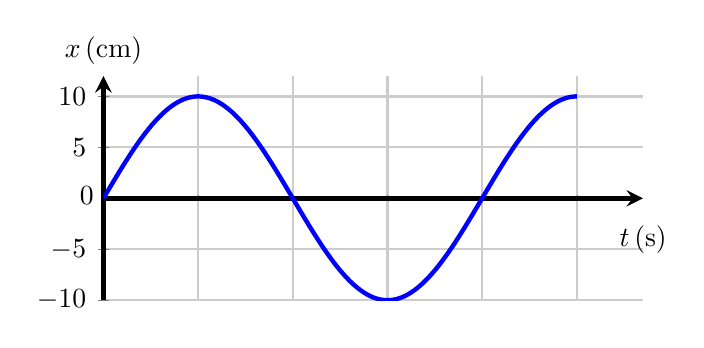
\begin{tikzpicture}  
			\begin{axis}[  ultra thick,
				xmin=0,  
				xmax=5.7, 
				ymin=-10,  
				ymax=12, 
				xtick={0,1,...,5},
				ytick={-10,-5,...,10},
				xticklabels=\empty,
%				minor x tick num=0,
%				minor y tick num=1,
				samples=300,
				axis lines=middle, 
				grid style={step=1, color=gray!20!white},
				grid=both,
				major grid style={line width=0.8pt,gray!40!white},
				xlabel=$\xsi{t}{\left(\second\right)}$, 
				ylabel=$\xsi{x}{\left(\si{\centi\meter}\right)}$, 
				every axis y label/.style={at=(current axis.above origin),anchor=south},  
				every axis x label/.style={at=(current axis.right of origin),anchor=east, below=1.5cm}, yscale=0.5 ]  
				\addplot [ultra thick, blue, smooth, domain=0:5] {10*cos(deg(pi*x/2-pi/2))}; 
			\end{axis}
		\node[label={[left]90:0}] at (0,1.2){};  
		\end{tikzpicture}
	\end{center}
	\choice
	{$\SI{20}{\centi\meter}$}
	{\True $\SI{10}{\centi\meter}$}
	{$\SI{5}{\centi\meter}$}
	{$\SI{30}{\centi\meter}$}
	\loigiai{}
\end{ex}
% ===================================================================
\begin{ex}
Một vật dao động điều hoà có đồ thị li độ - thời gian được mô tả như hình bên. Chu kì dao động của vật là	
	\begin{center}
		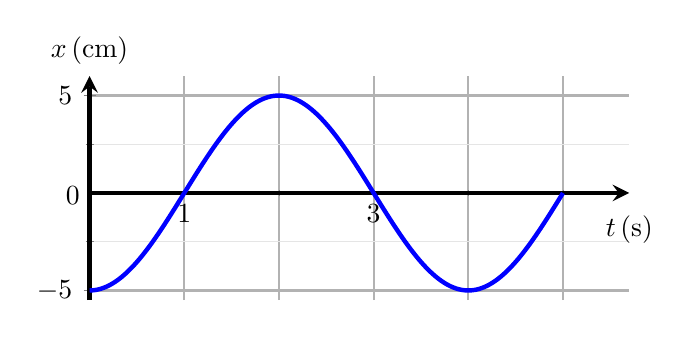
\begin{tikzpicture}  
			\begin{axis}[  ultra thick,
				xmin=0,  
				xmax=5.7, 
				ymin=-5.5,  
				ymax=6, 
				xtick={0,1,...,5},
				ytick={-5,0,5},
				xticklabels=\empty,
				%				minor x tick num=0,
							minor y tick num=1,
				samples=300,
				axis lines=middle, 
				grid style={step=1, color=gray!20!white},
				grid=both,
				major grid style={line width=0.8pt,gray!60!white},
				xlabel=$\xsi{t}{\left(\second\right)}$, 
				ylabel=$\xsi{x}{\left(\si{\centi\meter}\right)}$, 
				every axis y label/.style={at=(current axis.above origin),anchor=south},  
				every axis x label/.style={at=(current axis.right of origin),anchor=east, below=1.5cm}, yscale=0.5 ]  
				\addplot [ultra thick, blue, smooth, domain=0:5] {5*cos(deg(pi*x/2-pi))}; 
				\node at (axis cs:1,0) [below] {1};
				\node at (axis cs:3,0) [below] {3};
			\end{axis}
			\node[label={[left]90:0}] at (0,1.2){};  
		\end{tikzpicture}
	\end{center}
	\choice
	{$\SI{1}{\second}$}
	{$\SI{2}{\second}$}
	{\True $\SI{4}{\second}$}
	{$\SI{3}{\second}$}
	\loigiai{}
\end{ex}
% ===================================================================
\begin{ex}
Một vật dao động điều hoà với phương trình li độ $x=\xsi{4\cos\left(4\pi t-\dfrac{\pi}{4}\right)}{\centi\meter}$. Chu kì dao động của vật là	
	\choice
	{$\xsi{4\pi}{\second}$}
	{$\SI{2}{\second}$}
	{\True $\SI{0.5}{\second}$}
	{$\xsi{2\pi}{\second}$}
	\loigiai{}
\end{ex}
% ===================================================================
\begin{ex}
Một vật dao động điều hoà, trong thời gian 1 phút vật thực hiện được 20 dao động. Tần số dao động của vật là	
	\choice
	{\True $\xsi{\dfrac{1}{3}}{\hertz}$}
	{$\SI{3}{\hertz}$}
	{$\SI{120}{\hertz}$}
	{$\SI{20}{\hertz}$}
	\loigiai{}
\end{ex}
% ===================================================================
\begin{ex}
Cho vật dao động điều hoà có đồ thị li độ - thời gian được mô tả như hình bên. Thời gian giữa hai lần liên tiếp vật đi qua vị trí cân bằng là
	\begin{center}
		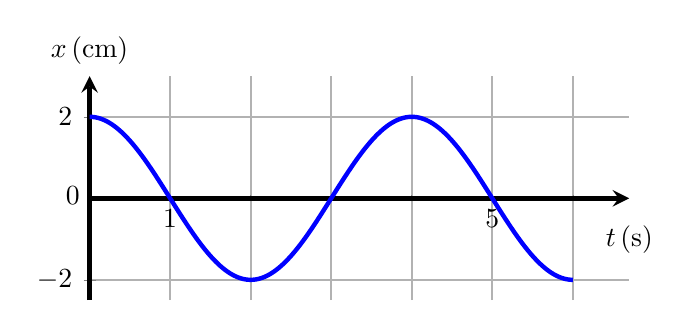
\begin{tikzpicture}  
			\begin{axis}[  ultra thick,
				xmin=0,  
				xmax=6.7, 
				ymin=-2.5,  
				ymax=3, 
				xtick={0,1,...,6},
				ytick={-2,0,2},
				xticklabels=\empty,
				%				minor x tick num=0,
				%minor y tick num=1,
				samples=300,
				axis lines=middle, 
				grid style={step=1, color=gray!20!white},
				grid=both,
				major grid style={line width=0.8pt,gray!60!white},
				xlabel=$\xsi{t}{\left(\second\right)}$, 
				ylabel=$\xsi{x}{\left(\si{\centi\meter}\right)}$, 
				every axis y label/.style={at=(current axis.above origin),anchor=south},  
				every axis x label/.style={at=(current axis.right of origin),anchor=east, below=1.5cm}, yscale=0.5 ]  
				\addplot [ultra thick, blue, smooth, domain=0:6] {2*cos(deg(pi*x/2))}; 
				\node at (axis cs:1,0) [below] {1};
				\node at (axis cs:5,0) [below] {5};
			\end{axis}
			\node[label={[left]90:0}] at (0,1.2){};  
		\end{tikzpicture}
	\end{center}
	\choice
	{$\SI{1}{\second}$}
	{$\SI{5}{\second}$}
	{$\SI{4}{\second}$}
	{\True $\SI{2}{\second}$}
	\loigiai{}
\end{ex}
% ===================================================================
\begin{ex}
	Cho hai vật dao động điều hoà với các phương trình li độ:
	$$x_1=\xsi{5\cos\left(3\pi t+\dfrac{\pi}{3}\right)}{\centi\meter}\quad \text{và}\quad x_2=\xsi{4\cos\left(3\pi t-\dfrac{\pi}{6}\right)}{\centi\meter}.$$ Độ lệch pha của hai dao động này là
	\choice
	{$\xsi{\dfrac{\pi}{3}}{\radian}$}
	{\True $\xsi{\dfrac{\pi}{2}}{\radian}$}
	{$\xsi{\dfrac{\pi}{6}}{\radian}$}
	{$\xsi{\dfrac{2\pi}{3}}{\radian}$}
	\loigiai{}
\end{ex}
% ===================================================================
\begin{ex}
Cho hai vật dao động điều hoà	cùng chu kì có đồ thị li độ - thời gian được mô tả như hình bên. Độ lệch pha giữa hai dao động là
\begin{center}
	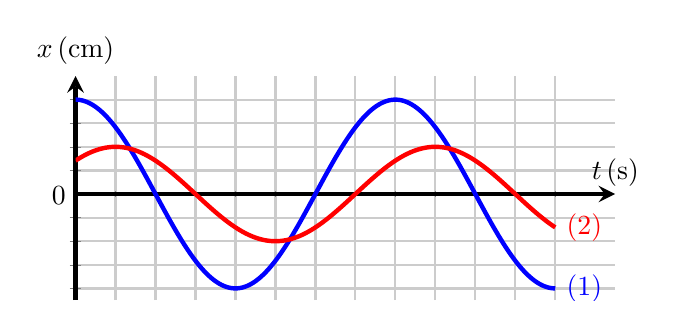
\begin{tikzpicture}  
		\begin{axis}[  ultra thick,
			xmin=0,  
			xmax=13.5, 
			ymin=-4.5,  
			ymax=5, 
			xtick={0,1,...,12},
			ytick={-4,-3,...,4},
			xticklabels=\empty,
			yticklabels=\empty,
			%				minor x tick num=0,
			%minor y tick num=1,
			samples=300,
			axis lines=middle, 
			grid style={step=1, color=gray!20!white},
			grid=both,
			major grid style={line width=0.8pt,gray!40!white},
			xlabel=$\xsi{t}{\left(\second\right)}$, 
			ylabel=$\xsi{x}{\left(\si{\centi\meter}\right)}$, 
			every axis y label/.style={at=(current axis.above origin),anchor=south},  
			every axis x label/.style={at=(current axis.right of origin),anchor=east, below=0.75cm}, yscale=0.5 ]  
			\addplot [ultra thick, blue, smooth, domain=0:12] {4*cos(deg(pi*x/4))} node [right] {(1)}; 
			\addplot [ultra thick, red, smooth, domain=0:12] {2*cos(deg(pi*x/4-pi/4))} node [right] {(2)};
		\end{axis}
		\node[label={[left]90:0}] at (0,1.2){};  
	\end{tikzpicture}
\end{center}
	\choice
	{\True $\xsi{\dfrac{\pi}{4}}{\radian}$}
	{$\xsi{\dfrac{\pi}{2}}{\radian}$}
	{$\xsi{2\pi}{\radian}$}
	{$\SI{0}{\radian}$}
	\loigiai{}
\end{ex}
% ===================================================================
\begin{ex}
Cho hai con lắc lò xo cùng dao động điều hoà có cùng tần số và cùng biên độ với phương trình li độ của con lắc thứ nhất $x_1=\xsi{4\cos\left(4\pi t+\dfrac{2\pi}{3}\right)}{\centi\meter}$. Biết thời gian con lắc thứ hai có cùng trạng thái với con lắc thứ nhất là muộn hơn $\SI{0.1}{\second}$. Phương trình dao động của con lắc thứ hai là	
	\choice
	{$x_2=\xsi{4\cos\left(4\pi t-\dfrac{\pi}{5}\right)}{\centi\meter}$}
	{$x_2=\xsi{4\cos\left(4\pi t+\dfrac{2\pi}{5}\right)}{\centi\meter}$}
	{$x_2=\xsi{4\cos\left(4\pi t-\dfrac{2\pi}{15}\right)}{\centi\meter}$}
	{$x_2=\xsi{4\cos\left(4\pi t+\dfrac{4\pi}{15}\right)}{\centi\meter}$}
	\loigiai{}
\end{ex}
% ===================================================================
\begin{ex}
	Cho hai vật dao động điều hoà cùng chu kì có đồ thị li độ - thời gian được mô tả như hình bên. Độ lệch pha giữa hai dao động là
	\begin{center}
		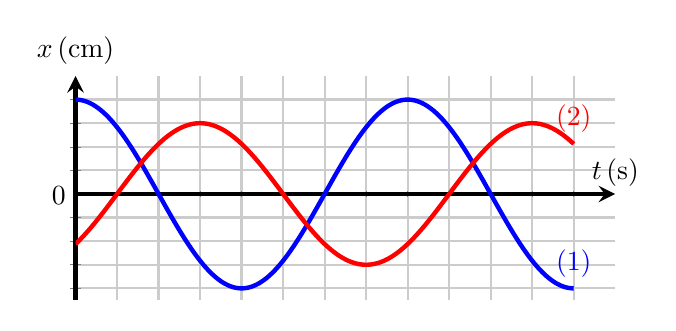
\begin{tikzpicture}  
			\begin{axis}[  ultra thick,
				xmin=0,  
				xmax=13, 
				ymin=-4.5,  
				ymax=5, 
				xtick={0,1,...,12},
				ytick={-4,-3,...,4},
				xticklabels=\empty,
				yticklabels=\empty,
				%				minor x tick num=0,
				%minor y tick num=1,
				samples=300,
				axis lines=middle, 
				grid style={step=1, color=gray!20!white},
				grid=both,
				major grid style={line width=0.8pt,gray!40!white},
				xlabel=$\xsi{t}{\left(\second\right)}$, 
				ylabel=$\xsi{x}{\left(\si{\centi\meter}\right)}$, 
				every axis y label/.style={at=(current axis.above origin),anchor=south},  
				every axis x label/.style={at=(current axis.right of origin),anchor=east, below=0.75cm}, yscale=0.5 ]  
				\addplot [ultra thick, blue, smooth, domain=0:12] {4*cos(deg(pi*x/4))} node [above] {(1)}; 
				\addplot [ultra thick, red, smooth, domain=0:12] {3*cos(deg(pi*x/4-3*pi/4))} node [above] {(2)};
			\end{axis}
			\node[label={[left]90:0}] at (0,1.2){};  
		\end{tikzpicture}
	\end{center}
	\choice
	{$\xsi{\dfrac{\pi}{4}}{\radian}$}
	{\True $\xsi{\dfrac{3\pi}{4}}{\radian}$}
	{$\xsi{2\pi}{\radian}$}
	{$\xsi{\dfrac{5\pi}{6}}{\radian}$}
	\loigiai{}
\end{ex}
\Closesolutionfile{ans}
\section{Tự luận}
\setcounter{ex}{0}
% ===================================================================
\begin{ex}
	Một vật dao động điều hoà có phương trình li độ $x=\xsi{2\cos\left(\pi t-\dfrac{\pi}{6}\right)}{\centi\meter}$, trong đó $t$ tính bằng giây. Trong $\SI{12}{\second}$ vật thực hiện được bao nhiêu dao động?
	\loigiai{$N=\dfrac{\Delta t}{T}=6$.}
\end{ex}
% ===================================================================
\begin{ex}
Xác định biên độ, chu kì, tần số và pha ban đầu của các dao động điều hoà sau:
\begin{enumerate}[label=\alph*)]
	\item $x=\xsi{5\cos\left(2\pi t-\dfrac{\pi}{2}\right)}{\centi\meter}$.
	\item $x=\xsi{-5\cos\left(\pi t-\dfrac{\pi}{6}\right)}{\centi\meter}$.
\end{enumerate}
	\loigiai{}
\end{ex}
% ===================================================================
\begin{ex}
	Một vật dao động điều hoà trên đoạn thẳng có chiều dài $\SI{4}{\centi\meter}$, vật thực hiện được 100 dao động trong $\SI{20}{\second}$. Tính biên độ, chu kì, tần số và tần số góc của dao động.
	\loigiai{}
\end{ex}
% ===================================================================
\begin{ex}
	Một vật dao động điều hoà với phương trình li độ $x=\xsi{5\cos\left(4\pi t+\dfrac{2\pi}{3}\right)}{\centi\meter}$, trong đó $t$ tính bằng giây.
	\begin{enumerate}[label=\alph*)]
		\item Xác định biên độ, tần số góc và pha ban đầu của dao động.
		\item Xác định chiều dài quỹ đạo của vật dao động.
		\item Xác định pha của dao động và li độ của vật tại các thời điểm $\SI{0.25}{\second}$ và $\SI{0.5}{\second}$.
	\end{enumerate}
	\loigiai{}
\end{ex}
% ===================================================================
\begin{ex}
	Một vật dao động điều hoà với phương trình li độ $x=\xsi{6\cos\left(3\pi t+\dfrac{\pi}{3}\right)}{\centi\meter}$ trong đó $t$ tính bằng giây. Lúc $t=\SI{2.0}{\second}$ thì các đại lượng sau đây có giá trị bằng bao nhiêu?
	\begin{enumerate}[label=\alph*)]
		\item Pha dao động.
		\item Li độ.
		\item Chu kì.
		\item Tần số.
	\end{enumerate}
	\loigiai{}
\end{ex}
% ===================================================================
\begin{ex}
	Đồ thị li độ - thời gian của hai vật dao động điều hoà $x_1\left(t\right)$ và $x_2\left(t\right)$ như hình vẽ. Xác định độ lệch pha giữa dao động của vật 1 so với dao động của vật 2.
	\begin{center}
		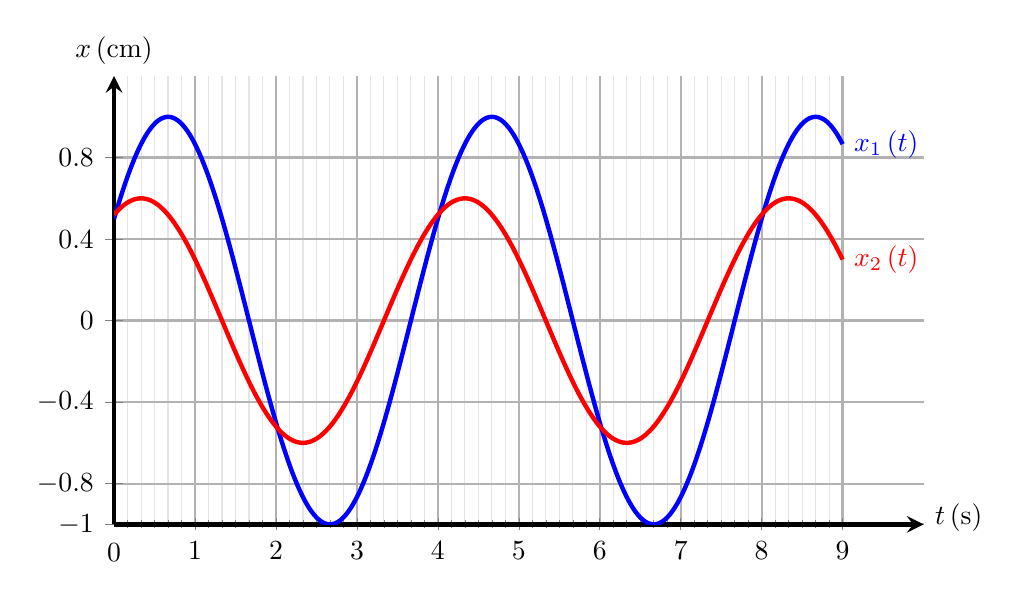
\begin{tikzpicture}  
			\begin{axis}[  ultra thick,
				xmin=0,  
				xmax=10, 
				ymin=-1,  
				ymax=1.2, 
				xtick={0,1,...,9},
				ytick={-1,-0.8,-0.4,0,0.4,0.8},
				minor x tick num=5,
				minor y tick num=1,
				samples=300,
				axis lines=middle, 
				axis x line shift={1},
				grid style={step=1, color=gray!20!white},
				grid=both,
				major grid style={line width=0.8pt,gray!60!white},
				xlabel=$\xsi{t}{\left(\second\right)}$, 
				ylabel=$\xsi{x}{\left(\si{\centi\meter}\right)}$, 
				every axis y label/.style={at=(current axis.above origin),anchor=south},  
				every axis x label/.style={at=(current axis.right of origin),below=2.5cm,anchor=west}, xscale=1.5]  
				\addplot [ultra thick, blue, smooth, domain=0:9] {1*cos(deg(pi*x/2-pi/3))} node [right] {$x_1\left(t\right)$}; 
				\addplot [ultra thick, red, smooth, domain=0:9] {0.6*cos(deg(pi*x/2-pi/6))} node [right] {$x_2\left(t\right)$};
			\end{axis}
		\node[label={[below]90:0}] at (0,-0.25){};
		\end{tikzpicture}
	\end{center}
	\loigiai{$\Delta \varphi=\xsi{\dfrac{\pi}{6}}{\radian}$.}
\end{ex}
% ===================================================================
\begin{ex}
	Đồ thị li độ - thời gian của 2 vật dao động điều hoà được thể hiện như hình vẽ.
		\begin{center}
		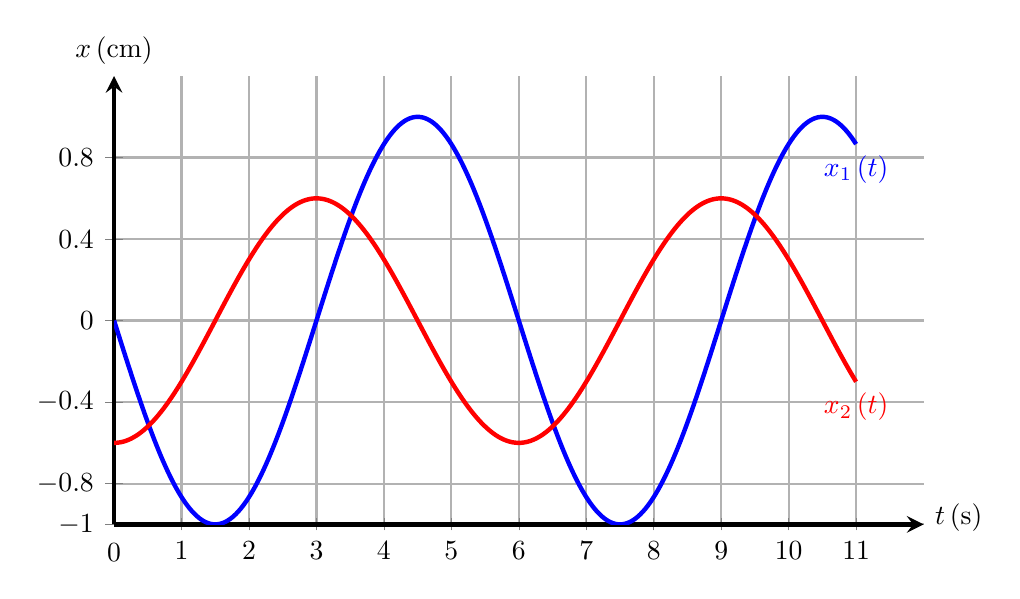
\begin{tikzpicture}  
			\begin{axis}[  ultra thick,
				xmin=0,  
				xmax=12, 
				ymin=-1,  
				ymax=1.2, 
				xtick={0,1,...,11},
				ytick={-1,-0.8,-0.4,0,0.4,0.8},
%				minor x tick num=5,
%				minor y tick num=1,
				samples=300,
				axis lines=middle, 
				axis x line shift={1},
				grid style={step=1, color=gray!20!white},
				grid=both,
				major grid style={line width=0.8pt,gray!60!white},
				xlabel=$\xsi{t}{\left(\second\right)}$, 
				ylabel=$\xsi{x}{\left(\si{\centi\meter}\right)}$, 
				every axis y label/.style={at=(current axis.above origin),anchor=south},  
				every axis x label/.style={at=(current axis.right of origin),below=2.5cm,anchor=west}, xscale=1.5]  
				\addplot [ultra thick, blue, smooth, domain=0:11] {1*cos(deg(pi*x/3+pi/2))} node [below] {$x_1\left(t\right)$}; 
				\addplot [ultra thick, red, smooth, domain=0:11] {0.6*cos(deg(pi*x/3-pi))} node [below] {$x_2\left(t\right)$};
			\end{axis}
			\node[label={[below]90:0}] at (0,-0.25){};
		\end{tikzpicture}
	\end{center}
	\begin{enumerate}[label=\alph*)]
		\item Xác định tần số của mỗi dao động.
		\item Cho biết dao động của vật 1 hay dao động của vật 2 đạt cực đại trước? Giải thích.
		\item Xác định độ lệch pha giữa dao động của vật 1 và dao động của vật 2.
	\end{enumerate}
	\loigiai{}
\end{ex}

%\tikzstyle{startstop} = [rectangle, rounded corners, minimum width=10cm, minimum height=1.5cm,text centered, draw=black, fill=green!20]
\begin{center}
	\begin{tikzpicture}
		\node (start) [startstop] {\bfseries \text{ÔN TẬP BÀI 1 VÀ BÀI 2}};
	\end{tikzpicture}
\end{center}
\setcounter{section}{0}
\section{Câu trắc nghiệm nhiều phương án lựa chọn}
\Opensolutionfile{ans}[ans/G12BT1+2TN]
% ===================================================================
\begin{ex}
	Với mô hình động học phân tử, sự khác biệt về cấu trúc của chất rắn, chất lỏng, chất khí là do sự khác biệt về
	\choice
	{thành phần các phân tử cấu tạo của mỗi chất}
	{\True độ lớn lực tương tác giữa các phân tử trong mỗi chất}
	{số lượng phân tử cấu tạo nên mỗi chất}
	{kích thước của các phân tử cấu tạo mỗi chất}
	\loigiai{}
\end{ex}
% ===================================================================
\begin{ex}
Khi nói về khoảng cách trung bình giữa các phân tử trong chất rắn, chất lỏng, chất khí. Kết luận nào sau đây là \textbf{đúng}?	
	\choice
	{Khoảng cách giữa các phân tử trong chất lỏng xa hơn so với các phân tử trong chất khí}
	{Khoảng cách giữa các phân tử trong chất rắn xa hơn so với các phân tử trong chất lỏng}
	{\True Khoảng cách giữa các phân tử trong chất lỏng gần hơn so với các phân tử trong chất khí}
	{Khoảng cách giữa các phân tử trong chất lỏng xa hơn so với các phân tử trong chất khí}
	\loigiai{}
\end{ex}
% ===================================================================
\begin{ex}
	Câu nào dưới đây nói về đặc tính của chất rắn kết tinh là \textbf{không đúng}?
	\choice
	{Các nguyên tử, phân tử liên kết chặt với nhau và sắp xếp theo một trật tự hình học xác định}
	{\True Không có nhiệt độ nóng chảy xác định}
	{Có cấu trúc tinh thể}
	{Có nhiệt độ nóng chảy xác định}
	\loigiai{}
\end{ex}
% ===================================================================
\begin{ex}
	Chất rắn nào dưới đây thuộc loại chất rắn vô định hình?
	\choice
	{Muối ăn}
	{Nhựa đường}
	{Kim loại}
	{Kim cương}
	\loigiai{}
\end{ex}
% ===================================================================
\begin{ex}
	Chất lỏng không có hình dạng xác định vì các phân tử chất lỏng
	\choice
	{dao động tại các vị trí cân bằng xác định}
	{có thể chuyển động phân tán ra xa nhau}
	{\True dao động quanh các vị trí cân bằng có thể dịch chuyển được}
	{có thể chuyển động tự do}
	\loigiai{}
\end{ex}
% ===================================================================
\begin{ex}
Chất khí dễ bị nén hơn so với chất rắn và chất lỏng vì	
	\choice
	{lực tương tác giữa các phân tử trong chất khí lớn hơn so với lực tương tác giữa các phân tử trong chất rắn và chất lỏng}
	{\True khoảng cách giữa các phân tử trong chất khí lớn hơn so với khoảng cách giữa các phân tử trong chất rắn và chất lỏng}
	{các phân tử trong chất khí ít chuyển động hơn so với các phân tử trong chất rắn và chất lỏng}
	{các phân tử trong chất khí có kích thước nhỏ hơn so với các phân tử trong chất rắn và chất lỏng}
	\loigiai{}
\end{ex}
% ===================================================================
\begin{ex}
Khi nói về quá trình nóng chảy và đông đặc là đang nói về quá trình chuyển thể giữa	
	\choice
	{chất rắn và chất khí}
	{chất khí và chất lỏng}
	{\True chất rắn và chất lỏng}
	{các chất bất kì}
	\loigiai{}
\end{ex}
% ===================================================================
\begin{ex}
	Quá trình chuyển từ thể khí sang thể rắn của các chất được gọi là
	\choice
	{\True sự ngưng kết}
	{thăng hoa}
	{sự đông đặc}
	{sự ngưng tụ}
	\loigiai{}
\end{ex}
% ===================================================================
\begin{ex}
	Khi chất rắn kết tinh được nung nóng. Kết luận nào sau đây là \textbf{đúng}?
	\choice
	{các phân tử vẫn dao động với biên độ không đổi, khoảng cách giữa các phân tử không đổi}
	{\True các phân tử dao động với biên độ tăng lên, khoảng cách giữa các phân tử tăng lên}
	{các phân tử dao động với biên độ không đổi, khoảng cách giữa các phân tử tăng lên}
	{các phân tử dao động với biên độ tăng lên, khoảng cách giữa các phân tử không đổi}
	\loigiai{}
\end{ex}
% ===================================================================
\begin{ex}
	Sự nóng chảy của chất rắn kết tinh bắt đầu xảy ra khi
	\choice
	{một số phân tử dao động mạnh hơn các phân tử xung quanh}
	{một số phân tử va chạm với các phân tử xung quanh}
	{một số phân tử dao động mạnh lên và truyền năng lượng dao động cho các phân tử khác}
	{\True một số phân tử thắng được lực liên kết với các phân tử xung quanh và thoát khỏi liên kết với chúng}
	\loigiai{}
\end{ex}
% ===================================================================
\begin{ex}
Trong quá trình chất rắn kết tinh đang nóng chảy nhiệt độ của nó không tăng thêm là do
	\choice
	{phần nhiệt nhận thêm cân bằng với phần nhiệt toả ra môi trường bên ngoài}
	{phần nhiệt lượng nhận thêm đã chuyển thành động năng của các phân tử}
	{\True phần nhiệt lượng nhận thêm đã chuyển thành năng lượng để tiếp tục phá vỡ liên kết của mạng tinh thể}
	{phần nhiệt lượng nhận thêm đã chuyển thành thế năng của các phân tử}
	\loigiai{}
\end{ex}
% ===================================================================
\begin{ex}
	Khi cho một cục nước đá vào nước ở nhiệt độ phòng thì kết luận nào sau đây là \textbf{đúng}?
	\choice
	{Nhiệt độ của nước trong cốc từ từ tăng lên}
	{Nước trong cốc sẽ nhận nhiệt lượng từ cục nước đá}
	{\True Nhiệt lượng được truyền từ nước trong cốc cho cục nước đá}
	{Quá trình truyền nhiệt kết thúc khi cục nước đá tan hết.}
	\loigiai{}
\end{ex}
% ===================================================================
\begin{ex}
	Có ba vật A, B, C có các nhiệt độ lần lượt là $t_\text{A}$, $t_\text{B}$, $t_\text{C}$. Cho vật A tiếp xúc với vật B đến khi cân bằng nhiệt, ngay sau đó lại cho vật A tiếp xúc với vật C đến khi cân bằng nhiệt thì nhiệt độ của vật A lúc này bằng với nhiệt độ của nó lúc ban đầu khi chưa tiếp xúc với các vật khác. Kết luận nào sau đây là \textbf{đúng}?
	\choice
	{Vật B đóng vai trò truyền nhiệt lượng khi tiếp xúc với vật A}
	{Vật C đóng vai trò nhận nhiệt lượng khi tiếp xúc với vật A}
	{Nhiệt độ của vật B thấp hơn nhiệt độ của vật C}
	{\True Tổng nhiệt lượng mà vật A nhận được bằng tổng nhiệt lượng mà nó truyền cho vật khác}
	\loigiai{}
\end{ex}
% ===================================================================
\begin{ex}
	Gọi $t_1$, $t_2$ lần lượt là nhiệt độ điểm đóng băng và nhiệt độ sôi của nước tinh khiết ở điều kiện áp suất tiêu chuẩn. Trong thang nhiệt độ Celsius, mỗi độ chia $\left(\SI{1}{\celsius}\right)$ có độ lớn bằng
	\choice
	{$100\left(t_2-t_1\right)$}
	{$100\left(t_1-t_2\right)$}
	{\True $\dfrac{1}{100}\left(t_2-t_1\right)$}
	{$\dfrac{1}{273,15}\left(t_2-t_1\right)$}
	\loigiai{}
\end{ex}
% ===================================================================
\begin{ex}
Nhiệt độ không tuyệt đối là nhiệt độ mà tại đó tất cả các chất có	
	\choice
	{động năng chuyển động nhiệt của các nguyên tử hoặc phân tử bằng không và thế năng của chúng là cực đại}
	{động năng chuyển động nhiệt của các nguyên tử hoặc phân tử là cực đại và thế năng của chúng là tối thiểu}
	{\True động năng chuyển động nhiệt của các nguyên tử hoặc phân tử bằng không và thế năng của chúng là tối thiểu}
	{động năng chuyển động nhiệt của các nguyên tử hoặc phân tử và thế năng của chúng là cực đại}
	\loigiai{}
\end{ex}
% ===================================================================
\begin{ex}
Gọi $\Delta t$ và $\Delta T$ lần lượt  là độ lớn một độ chia trên thang đo nhiệt độ Celsius và thang đo nhiệt độ Kelvin. Hệ thức nào sau đây là \textbf{đúng}?
	\choice
	{$\Delta t=\dfrac{1}{273}\Delta T$}
	{$\Delta t=273\Delta T$}
	{$\Delta T=\dfrac{1}{100}\Delta t$}
	{\True $\Delta T =\Delta t$}
	\loigiai{}
\end{ex}
% ===================================================================
\begin{ex}
Kết luận nào sau đây về nhiệt độ của một vật là \textbf{đúng}?	
	\choice
	{Nhiệt độ của một vật bất kì luôn có giá trị lớn hơn $\SI{0}{\celsius}$}
	{Nhiệt độ của một vật bất kì tỉ lệ thuận với khối lượng của nó}
	{Nhiệt độ của một vật bất kì phụ thuộc vào khoảng cách giữa các phân tử trong mạng tinh thể}
	{\True Nhiệt độ của một vật bất kì không thể nhỏ hơn $\SI{0}{\kelvin}$}
	\loigiai{}
\end{ex}
% ===================================================================
\begin{ex}
Một thang nhiệt độ Z có nhiệt độ đóng băng của nước là $-\SI{12}{\degree Z}$ và khoảng cách mỗi độ chia trong thang đo nhiệt độ Z có độ lớn bằng $\SI{0.8}{}$	lần khoảng cách một độ chia trong thang đo nhiệt độ Kelvin. Nhiệt độ sôi của nước trong thang nhiệt độ Z là
	\choice
	{\True $\SI{113}{\degree Z}$}
	{$\SI{137}{\degree Z}$}
	{$\SI{68}{\degree Z}$}
	{$\SI{92}{\degree Z}$}
	\loigiai{$\Delta t_Z=0,8\Delta T\Rightarrow \left(t_Z+12\right)=0,8\cdot 100\Rightarrow t_Z=\SI{113}{\degree Z}$.}
\end{ex}
% ===================================================================
\begin{ex}
Một thang đo nhiệt độ Y, trong đó nhiệt độ nước đá đang tan là $-\SI{25}{\degree Y}$ và nhiệt độ sôi của nước là $\SI{85}{\degree Y}$. Nhiệt độ $\SI{70}{\degree Y}$ sẽ gần đúng tương ứng với nhiệt độ trong thang nhiệt độ Kelvin là	
	\choice
	{\True $\SI{360}{\kelvin}$}
	{$\SI{377}{\kelvin}$}
	{$\SI{350}{\kelvin}$}
	{$\SI{366}{\kelvin}$}
	\loigiai{
$\dfrac{t_Y+25}{85+25}=\dfrac{T-273}{100}$.	
}
% ===================================================================
\begin{ex}
Có hai thang đo nhiệt độ X và Y liên hệ với nhau theo công thức $T_\text{X}=\dfrac{3}{4}T_\text{Y}+20$. Độ biến thiên nhiệt độ $\SI{30}{\degree X}$ trong thang nhiệt X sẽ tương ứng với một độ biến thiên trong thang nhiệt Y là	
	\choice
	{$\SI{66.6}{\degree Y}$}
	{\True $\SI{40}{\degree Y}$}
	{$\SI{60}{\degree Y}$}
	{$\SI{86.6}{\degree Y}$}
	\loigiai{}
\end{ex}
\end{ex}
\Closesolutionfile{ans}
\section{Trắc nghiệm đúng/sai}
\setcounter{ex}{0}
\Opensolutionfile{ans}[ans/G12B1+2TF]
% ===================================================================
\begin{ex}
	Khi nung nóng một chất rắn kết tinh ở áp suất tiêu chuẩn, nhiệt độ của chất rắn tăng lên đến một giá trị nào đó thì chất rắn bắt đầu chuyển sang thể lỏng. Quá trình này được gọi là quá trình nóng chảy.
	\choiceTF[t]
	{\True Nhiệt độ mà chất rắn kết tinh bắt đầu nóng chảy gọi là nhiệt độ nóng chảy}
	{\True Trong quá trình nung nóng, các phân tử của chất rắn sẽ dao động mạnh làm tăng khoảng cách giữa chúng}
	{Nhiệt độ của chất rắn kết tinh tăng liên tục trong quá trình nung nóng đến khi nó nóng chảy hoàn toàn}
	{\True Sau khi chuyển sang thể lỏng, nếu ngừng cung cấp nhiệt lượng thì chất lỏng sẽ bắt đầu quá trình đông đặc}
	\loigiai{}
\end{ex}
% ===================================================================
\begin{ex}
\immini{
Máy thuỷ lực là một thiết bị quan trọng trong ngành xây dựng, kỹ thuật ô tô, \dots. Bên trong máy thuỷ lực người ta dùng một chất lỏng (dầu thuỷ lực). Khi ta tác dụng một lực $f$ lên piston nhỏ có diện tích $s$ lực này gây ra áp suất $p=f/s$ và được truyền nguyên vẹn đến piston lớn có diện tích $S$ và gây ra lực nâng $F$.	
}
{
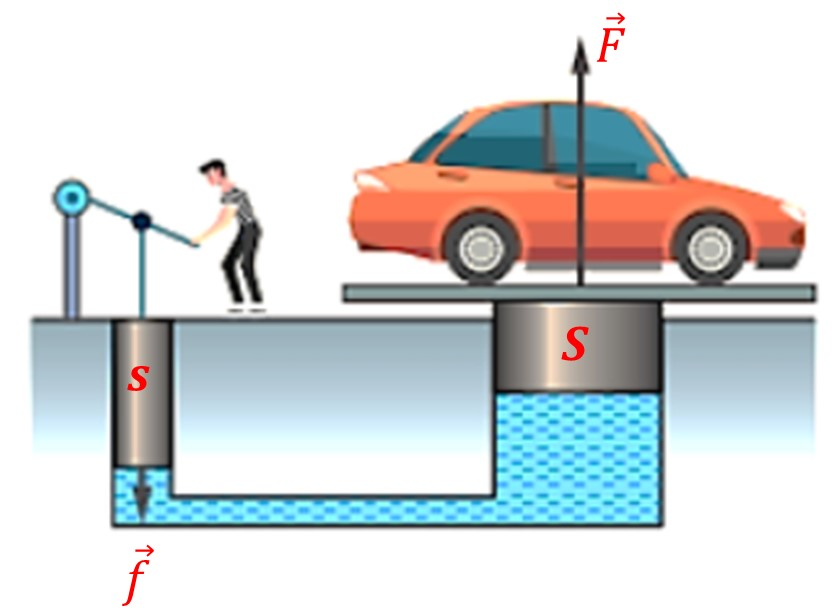
\includegraphics[width=0.6\linewidth]{figs/G12-BT1+2-1}
}
	\choiceTF[t]
	{Có thể thay thế chất lỏng trong máy thuỷ lực bằng chất khí}
	{Người ta sử dụng dầu thuỷ lực vì dầu thuỷ lực có đặc tính rất khó bị nén}
	{\True Nếu người ta nén với lực $f$ rất lón, các phân tử chất lỏng trong máy thuỷ lực càng bị nén chặt và có thể chuyển sang thể rắn}
	{Giả sử piston lớn có diện tích gấp 50 lần piston nhỏ. Khi đó, nếu muốn nâng một xe có khối lượng $\SI{1500}{\kilogram}$ thì cần tác dụng lên piston nhỏ một lực $\SI{30}{\newton}$}
	\loigiai{
\begin{itemchoice}
	\itemch Sai. Vì chất khí dễ bị nén nên máy không hoạt động được.
	\itemch Đúng.
	\itemch Sai. Chất lỏng không thể chuyển thành thể rắn khi chỉ bị nén.
	\itemch Sai. $p=\dfrac{f}{s}=\dfrac{F}{S}\Rightarrow f=\dfrac{Fs}{S}=\SI{300}{\newton}$.
	
	\end{itemchoice}	
}
\end{ex}
% ===================================================================
\begin{ex}

\immini{
Để tạo ra các loại rượu truyền thống đặc trưng của Việt Nam, các cơ sở sản xuất rượu đã thực hiện nhiều công đoạn. Trong các công đoạn đó có một công đoạn rất quan trọng là quá trình chưng cất rượu. Quá	trình chưng cất được thể hiện đơn giản bằng sơ đồ hình bên.
}
{
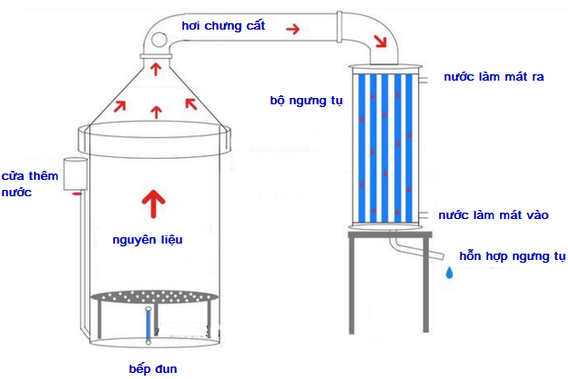
\includegraphics[width=0.7\linewidth]{figs/G12-BT1+2-2}
}
	\choiceTF[t]
	{\True Ở bồn A hỗn hợp nguyên liệu lỏng được cung cấp nhiệt lượng để tạo hơi rượu}
	{Rượu có nhiệt độ sôi cao hơn nước nên rượu hoá hơi trước}
	{Nước làm mát ở bồn B có tác dụng cung cấp nhiệt lượng cho quá trình ngưng tụ của hơi rượu}
	{\True Thực ra trong hỗn hợp hơi vừa có hơi rượu vừa có hơi nước}
	\loigiai{}
\end{ex}
% ===================================================================
\begin{ex}
	\immini{
Máy làm lạnh là một thiết bị khá quen thuộc trong đời sống hằng ngày. Nguyên tắc hoạt động của máy dựa trên nguyên tắc chuyển thể của môi chất gas bên trong máy. Sự trao đổi nhiệt với môi trường diễn ra ở giàn nóng và giàn lạnh của máy.	
}
{
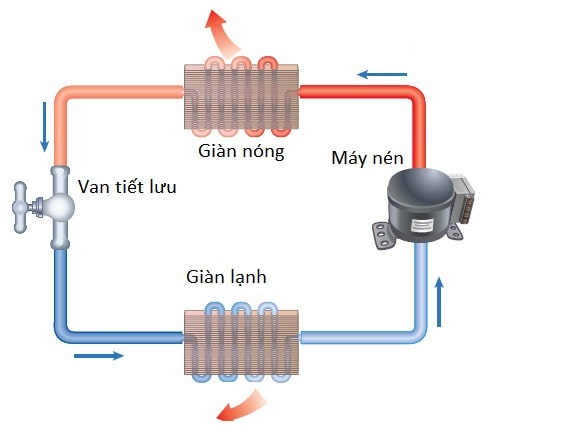
\includegraphics[width=0.65\linewidth]{figs/G12-BT1+2-3}
}
	\choiceTF[t]
	{\True Tại giàn nóng, gas có sự chuyển thể từ dạng khí sang lỏng}
	{\True Tại giàn lạnh, gas có sự chuyển thể từ dạng lỏng sang khí}
	{Tại giàn nóng, gas đã thu nhiệt từ môi trường}
	{Tại giàn lạnh, gas đã toả nhiệt ra môi trường}
	\loigiai{}
\end{ex}
% ===================================================================
\begin{ex}
	Hình bên là đồ thị phác hoạ sự thay đổi nhiệt độ theo thời gian trong quá trình chuyển thể từ rắn sang lỏng của chất rắn kết tinh và chất rắn vô định hình.
\begin{center}
	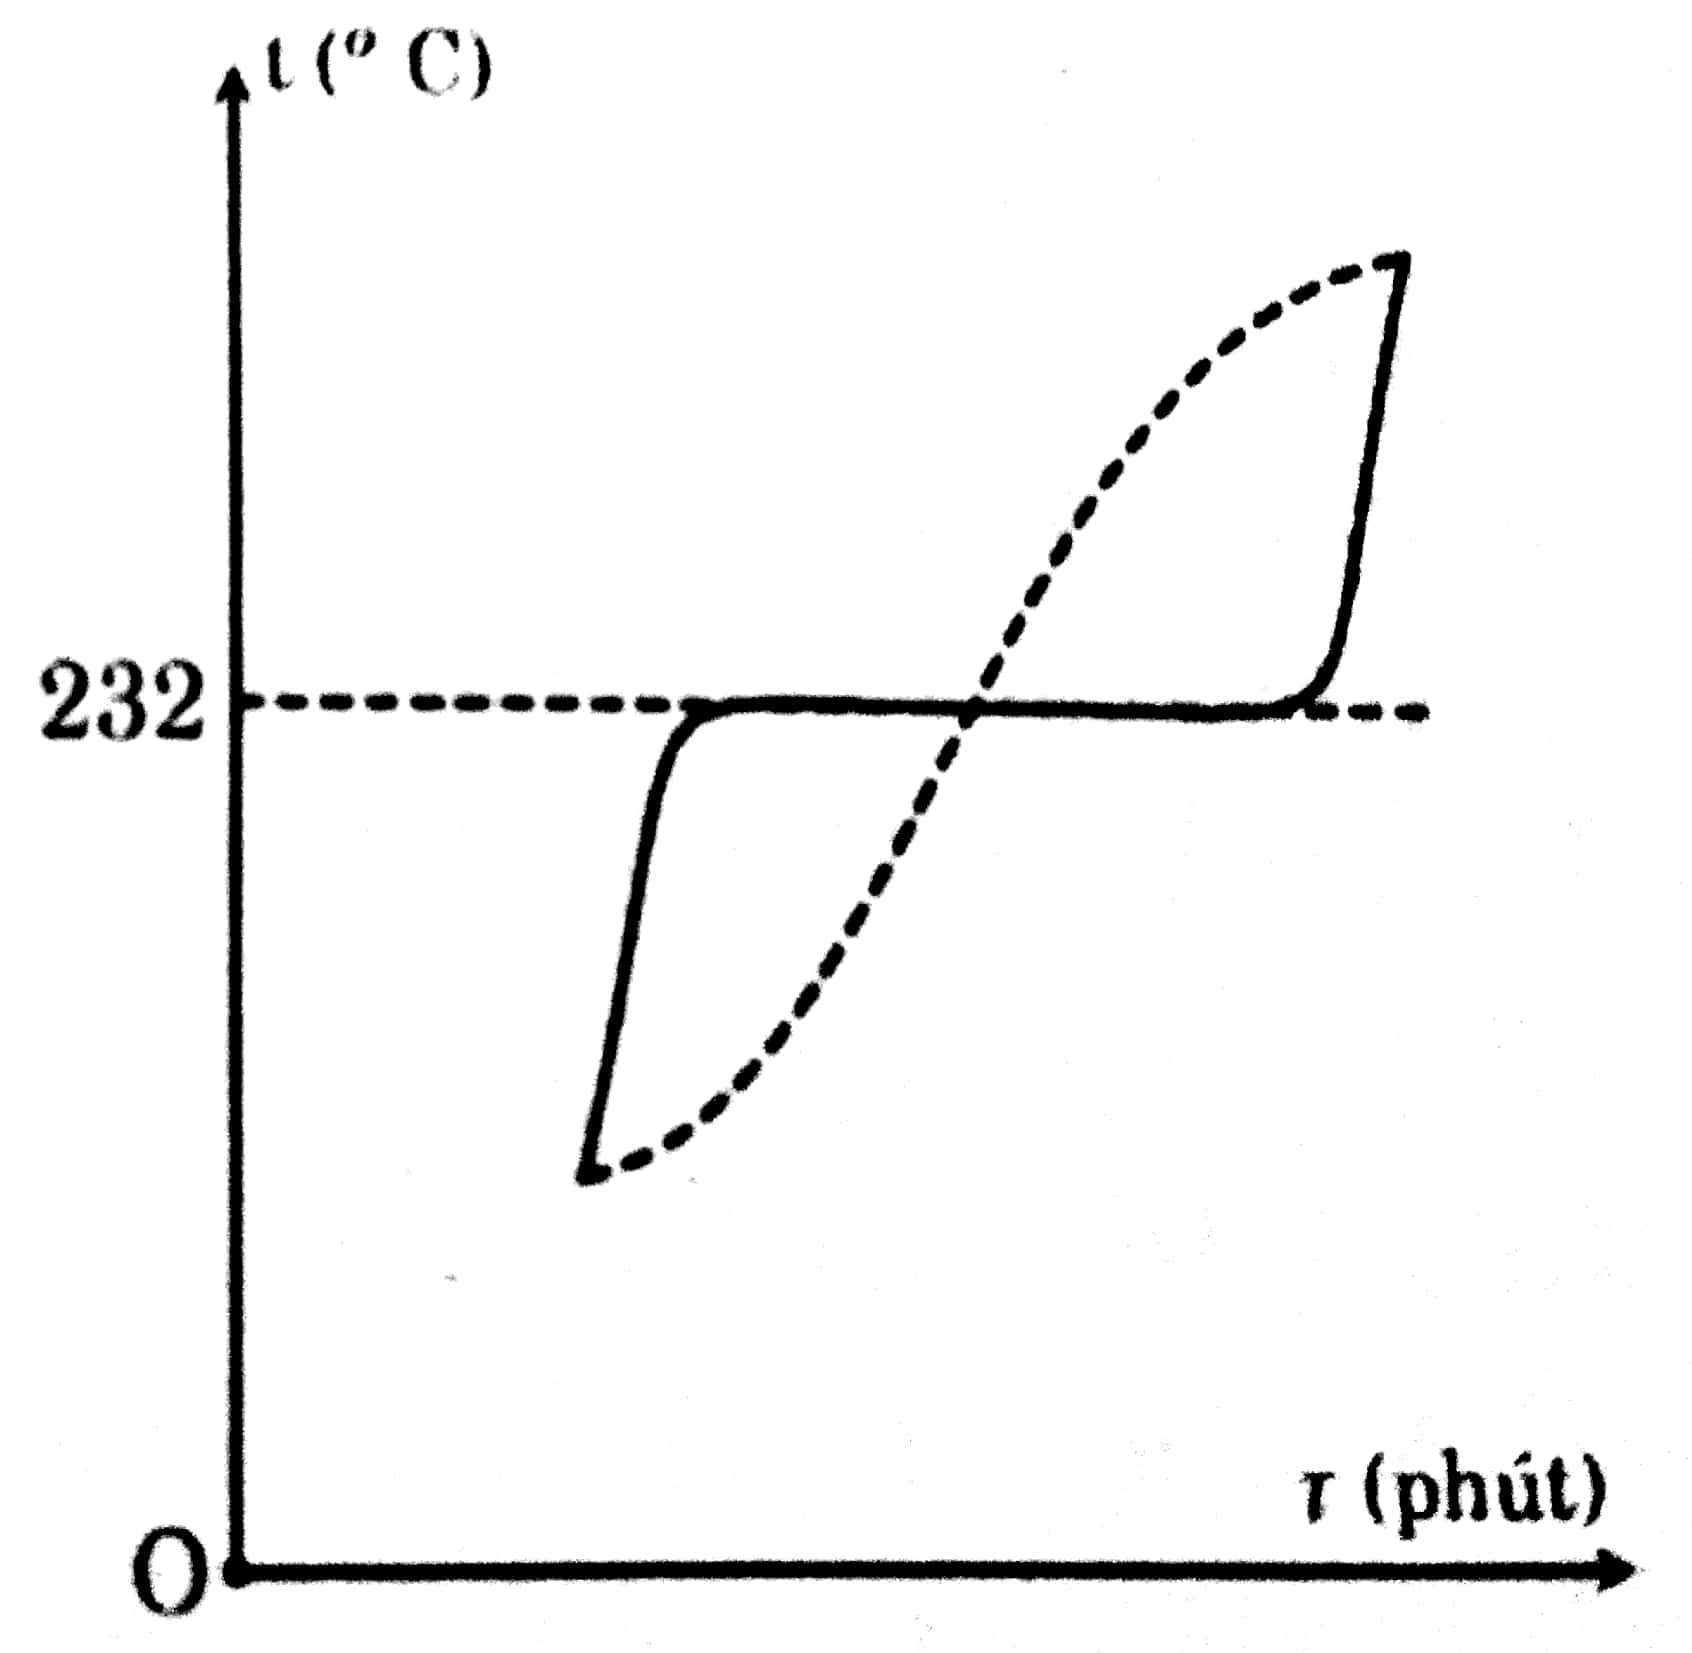
\includegraphics[width=0.3\linewidth]{figs/G12-BT1+2-4}
\end{center}
	\choiceTF[t]
	{Đường nét liền mô tả quá trình chuyển thể của chất rắn vô định hình}
	{Đường nét đứt mô tả quá trình chuyển thể của chất rắn kết tinh}
	{\True Nhiệt độ nóng chảy của chất rắn kết tinh là $\SI{232}{\celsius}$}
	{Chất rắn vô định hình có nhiệt độ nóng chảy cao hơn chất rắn kết tinh}
	\loigiai{}
\end{ex}

% ===================================================================
\begin{ex}
Có hai chai nước lạnh A và B giống nhau (cùng nhiệt độ, cùng thể tích).
\begin{enumerate}[label=\bfseries\itshape Lần \arabic*:, leftmargin=1.5cm]
	\item Nhúng chai A vào chậu nước, nhiệt độ nước trong chậu giảm xuống. Đến khi hệ cân bằng nhiệt thì lấy chai A ra khỏi chậu.
	\item Nhúng chai nước B vào chậu nước, nhiệt độ nước trong chậu tiếp tục giảm xuống đến khi cân bằng nhiệt thì lấy chai nước B ra khỏi chậu.
\end{enumerate}
	\choiceTF[t]
	{\True Nhiệt độ của chai nước A sau khi lấy ra khỏi chậu cao hơn nhiệt độ chai nước B}
	{Nhiệt lượng của chậu nước truyền cho hai chai nước là như nhau}
	{\True Độ giảm nhiệt độ của chậu nước trong lần nhúng thứ nhất nhiều hơn lần nhúng thứ hai}
	{Tổng độ tăng nhiệt độ của hai chai nước bằng tổng độ giảm nhiệt độ của chậu nước trong hai lần nhúng}
	\loigiai{}
\end{ex}
% ===================================================================
\begin{ex}
	Hình bên mô tả mối liên hệ giữa hai thang đo nhiệt độ Kelvin và Fahrenheit ở điều kiện áp suất tiêu chuẩn.
	\begin{center}
		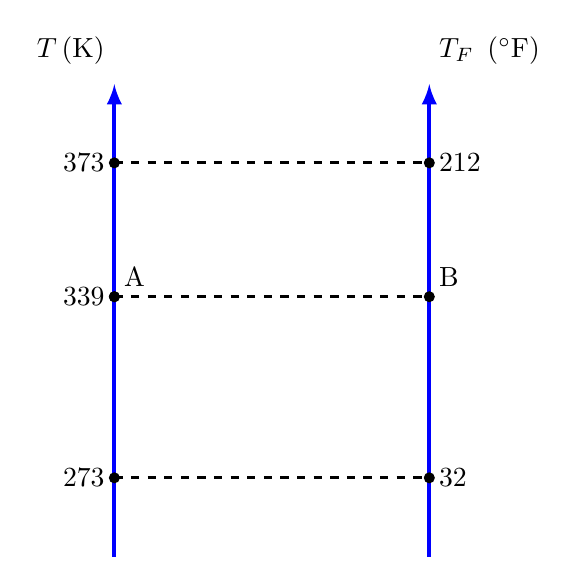
\begin{tikzpicture}
			\draw[line width=1.5pt, blue, -latex] (0,0)--(0,6);
			\draw[line width=1.5pt, blue, -latex] (4,0)--(4,6);
			\draw[line width=1pt, dashed] (0,1)--(4,1);
			\draw[line width=1pt, dashed] (0,5)--(4,5);
			\draw[line width=1pt, dashed] (0,3.3)--(4,3.3);
			\fill   (0,1) circle[radius=2pt]  node [left] {$273$};
			\fill   (4,1) circle[radius=2pt]  node [right] {$32$};
			\fill   (0,5) circle[radius=2pt]  node [left] {$373$};
			\fill   (4,5) circle[radius=2pt]  node [right] {$212$};
			\fill   (0,3.3) circle[radius=2pt]  node [left] {$339$};
			\fill   (0,3.3) circle[radius=2pt]  node [above right] {A};
			\fill   (4,3.3) circle[radius=2pt]  node [above right] {B};
			\node[label={[above left]90:$\xsi{T}{\left(\kelvin\right)}$}] at (0,6){};
			\node[label={[above right]90:$T_F\ \left(\si{\degree F}\right)$}] at (4,6){};
		\end{tikzpicture}
	\end{center}
	\choiceTF[t]
	{Mỗi độ chia trong thang đo nhiệt độ Fahrenheit có độ lớn bằng 1,8 lần mỗi độ chia trong thang đo nhiệt độ Kelvin}
	{\True Độ biến thiên nhiệt độ là $\SI{100}{\kelvin}$ trên thang đo nhiệt độ Kelvin sẽ tương ứng với độ biến thiên $\SI{180}{\degree F}$ trên thang đo nhiệt độ Fahrenheit}
	{\True Tại điểm B trên hình theo thang nhiệt độ Fahrenheit có nhiệt độ là $\SI{150.8}{\degree F}$}
	{\True Tại nhiệt độ $\SI{574.25}{}$ độ thì giá trị trên hai thang đo là bằng nhau}
	\loigiai{}
\end{ex}
% ===================================================================
\begin{ex}
Người ta dùng lò nấu chảy kim loại để nấu chảy sắt. Hình bên là đồ thị ghi lại sự thay đổi nhiệt độ của sắt theo thời gian.
\begin{center}
	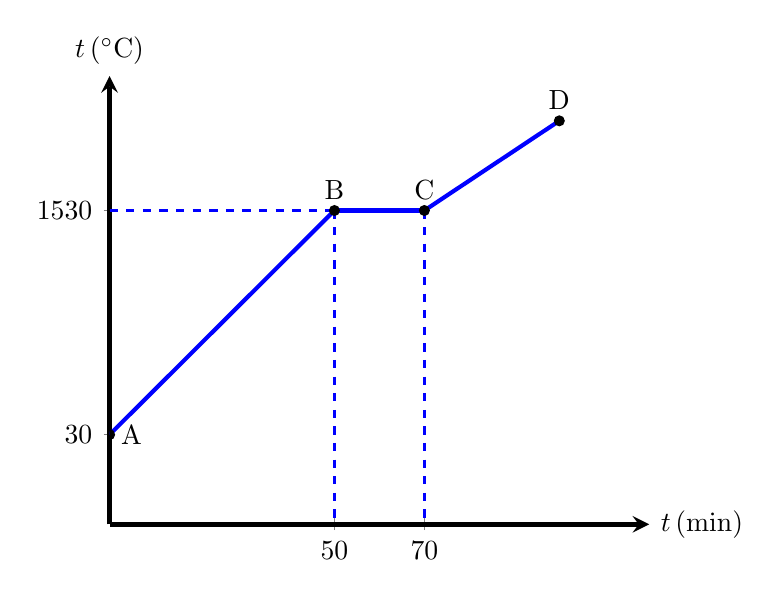
\begin{tikzpicture}  
		\begin{axis}[  ultra thick,
			xmin=0,  
			xmax=12,  
			xtick={0,5, 7},
			ytick={0,2,7},
%			minor x tick num=3,
%			minor y tick num=1,
			ymin=0,  
			ymax=10, 
			xticklabels={0,50,70},
			yticklabels={0,30,1530},
			samples=300,
			axis lines=middle, 
%			grid style={step=1,line width=0.4pt, color=gray!20!white},
%			grid=both,
%			major grid style={line width=0.8pt,gray!60!white},
			xlabel=$\xsi{t}{\left(\minute\right)}$, 
			ylabel=$\xsi{t}{\left(\si{\celsius}\right)}$, 
			every axis y label/.style={at=(current axis.above origin),anchor=south},  
			every axis x label/.style={at=(current axis.right of origin),anchor=west}]  
			\draw[line width=1.5pt, blue] (axis cs: 0,2)--(axis cs: 5,7);
			\draw[line width=1.5pt, blue] (axis cs: 5,7)--(axis cs: 7,7);
			\draw[line width=1.5pt, blue] (axis cs: 7,7)--(axis cs: 10,9);
			\draw[line width=1pt, dashed, blue] (axis cs: 5,7)--(axis cs: 5,0);
			\draw[line width=1pt, dashed, blue] (axis cs: 7,7)--(axis cs: 7,0);
			\draw[line width=1pt, dashed, blue] (axis cs: 0,7)--(axis cs: 5,7);
			\fill   (axis cs: 0,2) circle[radius=2pt]  node [right] {A};
			\fill   (axis cs: 5,7) circle[radius=2pt]  node [above] {B};
			\fill   (axis cs: 7,7) circle[radius=2pt]  node [above] {C};
			\fill   (axis cs: 10,9) circle[radius=2pt]  node [above] {D};
		\end{axis}  
	\end{tikzpicture}
\end{center}	
	\choiceTF[t]
	{\True Kể từ thời điểm ban đầu đến phút thứ 50, sắt vẫn ở thể rắn}
	{\True Nhiệt độ nóng chảy của sắt là $\SI{1530}{\celsius}$}
	{\True Từ phút thứ 50 đến phút thứ 70 là giai đoạn chuyển từ thể rắn sang thể lỏng}
	{Đoạn CD trên đồ thị thể hiện quá trình sôi của sắt}
	\loigiai{}
\end{ex}
% ===================================================================
\begin{ex}
	Giả sử có một thang đo nhiệt độ Z với nhiệt độ điểm đóng băng của nước tinh khiết là $-\SI{10}{\degree Z}$ và nhiệt độ sôi là $\SI{140}{\degree Z}$, biết rằng trong thang nhiệt độ Celsius nhiệt độ các điểm trên là $\SI{0}{\celsius}$ và $\SI{100}{\celsius}$ (các nhiệt độ đều được ghi nhận ở điều kiện áp suất tiêu chuẩn)
	\choiceTF[t]
	{\True Khoảng cách mỗi độ chia trong hai thang đo nhiệt độ là khác nhau}
	{Nếu độ biến thiên nhiệt độ là $\SI{10}{\celsius}$ trong thang nhiệt độ Celsius tương ứng với độ biến thiên $\SI{25}{\degree Z}$ trong thang nhiệt độ Z}
	{\True Nhiệt độ giữa hai thang đo nhiệt độ liên hệ với nhau $t=\dfrac{2}{3}T_\text{Z}+\dfrac{20}{3}$}
	{Nhiệt độ cơ thể người là $\SI{37}{\celsius}$ theo thang nhiệt Celsius thì tương ứng với nhiệt độ $\SI{55.5}{\degree Z}$}
	\loigiai{}
\end{ex}
\Closesolutionfile{ans}
%\tikzstyle{startstop} = [rectangle, rounded corners, minimum width=10cm, minimum height=1.5cm,text centered, draw=black, fill=green!20]
\begin{center}
	\begin{tikzpicture}
		\node (start) [startstop] {\bfseries \text{ÔN TẬP TUẦN 4}};
	\end{tikzpicture}
\end{center}
\setcounter{section}{0}
\Opensolutionfile{ans}[ans/G10TUAN4-TN]
% ===================================================================
\begin{ex}
	Chọn đáp án có từ /cụm từ thích hợp để hoàn thành bảng sau:
	\begin{center}
		\begin{tabular}{|c|c|c|}
			\hline
			\bfseries Đơn vị &\bfseries Kí hiệu & \bfseries Đại lượng\\
			\hline
			kelvin & (1) & (2)\\
			\hline
			ampe & $\si{\ampere}$ & (3)\\
			\hline
			candela & $\si{\candela}$ & (4)\\
			\hline
		\end{tabular}
	\end{center}
	\choice
	{(1) $\si{\kelvin}$; (2) Khối lượng; (3) Cường độ dòng điện; (4) Lượng chất}
	{\True (1) $\si{\kelvin}$; (2) Nhiệt độ; (3) Cường độ dòng điện; (4) Cường độ ánh sáng}
	{(1) $\si{\kelvin}$; (2) Nhiệt độ; (3) Cường độ dòng điện; (4) Lượng chất}
	{(1) $\si{\kelvin}$; (2) Khối lượng; (3) Cường độ dòng điện; (4) Cường độ ánh sáng}
	\loigiai{}
\end{ex}
% ===================================================================
\begin{ex}
	Đơn vị nào sau đây không thuộc thứ nguyên $L$ [Chiều dài]?
	\choice
	{Dặm}
	{Hải lí}
	{Năm ánh sáng}
	{\True Năm}
	\loigiai{}
\end{ex}
% ===================================================================
\begin{ex}
Đáp án nào sau đây có 1 đơn vị cơ bản và 1 đơn vị dẫn xuất?	
	\choice
	{mét, kilogram}
	{\True newton, mol}
	{pascal, joule}
	{candela, kelvin}
	\loigiai{}
\end{ex}
% ===================================================================
\begin{ex}
	Hãy chọn câu phát biểu \textbf{đúng}?
	\choice
	{Hệ quy chiếu bao gồm hệ toạ độ, mốc thời gian và đồng hồ}
	{Hệ quy chiếu bao gồm vật làm mốc, mốc thời gian và đồng hồ}
	{Hệ quy chiếu bao gồm vật làm mốc, hệ toạ độ, mốc thời gian}
	{\True Hệ quy chiếu bao gồm vật làm mốc, hệ toạ độ, mốc thời gian và đồng hồ}
	\loigiai{}
\end{ex}
% ===================================================================
\begin{ex}
Kết luận nào sau đây là \textbf{đúng} khi nói về độ dịch chuyển và quãng đường đi được của một vật?	
	\choice
	{Độ dịch chuyển và quãng đường đi được đều là đại lượng vô hướng}
	{\True Độ dịch chuyển là đại lượng vector còn quãng đường đi được là đại lượng vô hướng}
	{Độ dịch chuyển và quãng đường đi được đều là đại lượng vector}
	{Độ dịch chuyển và quãng đường đi được đều là đại lượng không âm}
	\loigiai{}
\end{ex}
% ===================================================================
\begin{ex}
	Khi vật chuyển động thẳng đều cùng chiều dương thì đồ thị $d - t$ của vật có dạng là
	\choice
	{đường thẳng vuông góc với trục $Od$}
	{\True đường thẳng xiên góc đi lên}
	{đường thẳng xiên góc đi xuống}
	{đường thẳng vuông góc với trục $Ot$}
	\loigiai{}
\end{ex}
% ===================================================================
\begin{ex}
	Cho đồ thị độ dịch chuyển – thời gian của một vật như hình. Chọn phát biểu \textbf{đúng}.	
	\begin{center}
		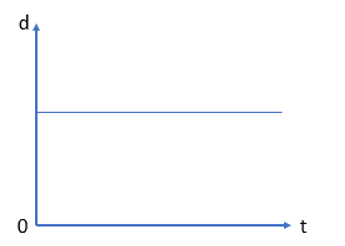
\includegraphics[width=0.25\linewidth]{figs/VN10-2023-PH-TP005-P-1}
	\end{center}
	\choice
	{Vật đang chuyển động thẳng đều theo chiều dương}
	{Vật đang chuyển động thẳng đều theo chiều âm}
	{\True Vật đang đứng yên}
	{Vật chuyển động thẳng đều theo chiều dương rồi đổi chiều chuyển động ngược lại}
	\loigiai{}
\end{ex}

% ===================================================================
\begin{ex}
Một vật bắt đầu chuyển động từ điểm O đến điểm A, sau đó chuyển động về điểm B. Quãng đường và độ dịch chuyển của vật tương ứng là	
\begin{center}
	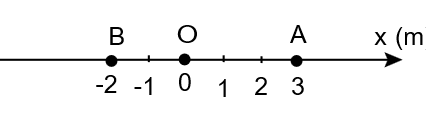
\includegraphics[width=0.4\linewidth]{figs/VN10-2022-PH-TP004-P-2}
\end{center}
	\choice
	{$\SI{2}{\meter}$; $\SI{-2}{\meter}$}
	{\True $\SI{8}{\meter}$; $\SI{-2}{\meter}$}
	{$\SI{2}{\meter}$; $\SI{2}{\meter}$}
	{$\SI{8}{\meter}$; $\SI{-8}{\meter}$}
	\loigiai{}
\end{ex}
% ===================================================================
\begin{ex}
“Lúc 15 giờ 30 phút hôm qua, xe chúng tôi đang chạy trên quốc lộ 5, cách Hải Dương 10 km”. Việc xác định vị trí của ô tô như trên còn thiếu yếu tố gì?	
	\choice
	{Vật làm mốc}
	{\True Chiều dương trên đường đi}
	{Mốc thời gian}
	{Thước đo và đồng hồ}
	\loigiai{}
\end{ex}

% ===================================================================
\begin{ex}

Hai người đi xe đạp từ A đến C, người thứ nhất đi theo đường từ A đến B, rồi từ B đến C; người thứ hai đi thẳng từ A đến C. Cả hai đều về đích cùng một lúc.\\
Hãy chọn kết luận \textbf{sai}.	
\immini{
	\choice
	{Người thứ nhất đi được quãng đường $\SI{8}{\kilo\meter}$}
	{Độ dịch chuyển của người thứ nhất và người thứ hai bằng nhau}
	{\True Độ dịch chuyển và quãng đường đi được của người thứ nhất bằng nhau}
	{Độ dịch chuyển của người thứ nhất là $\SI{5.7}{\kilo\meter}$, hướng $\SI{45}{\degree}$ Đông – Bắc}
}
	{
		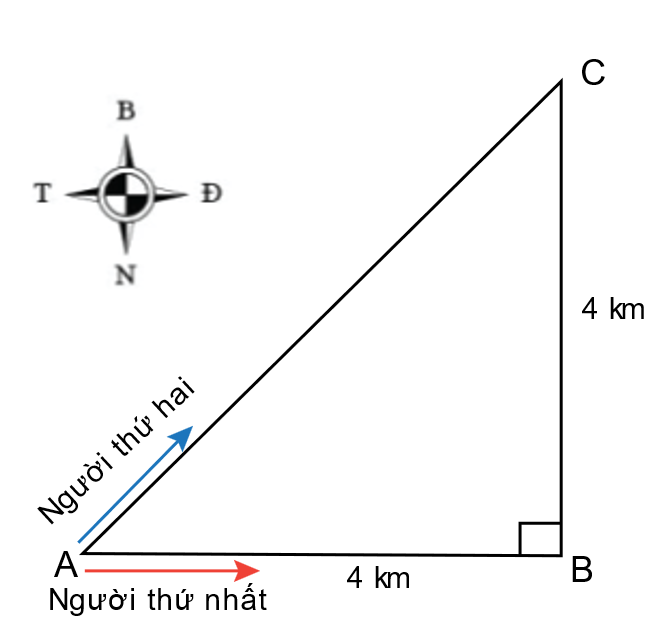
\includegraphics[width=0.5\linewidth]{figs/VN10-2022-PH-TP004-P-3}
	}
	\loigiai{}
	
\end{ex}
% ===================================================================
\begin{ex}
	Khi nhìn vào tốc kế của ô tô đang chạy, số chỉ trên tốc kế cho ta biết
	\choice
	{gia tốc tức thời của ô tô}
	{vận tốc tức thời của ô tô}
	{\True tốc độ tức thời của ô tô}
	{tốc độ trung bình của ô tô}
	\loigiai{}
\end{ex}
% ===================================================================
\begin{ex}
	Một máy bay phản lực có tốc độ $\SI{700}{\kilo\meter/\hour}$. Nếu muốn bay liên tục trên khoảng cách $\SI{1400}{\kilo\meter}$ thì máy bay phải bay trong thời gian là
	\choice
	{\True $\SI{2}{\hour}$}
	{$\SI{3}{\hour}$}
	{$\SI{2}{\hour}\SI{30}{\minute}$}
	{$\SI{1}{\hour}\SI{30}{\minute}$}
	\loigiai{Thời gian máy bay bay quãng đường $\SI{1400}{\kilo\meter}$:
		$$t=\dfrac{s}{v}=\SI{2}{\hour}.$$}
\end{ex}
% ===================================================================
\begin{ex}
	Đồ thị độ dịch chuyển – thời gian trong chuyển động thẳng của một chất điểm có dạng như hình vẽ.\\
	Trong thời gian nào xe chuyển động thẳng đều?
	\begin{center}
		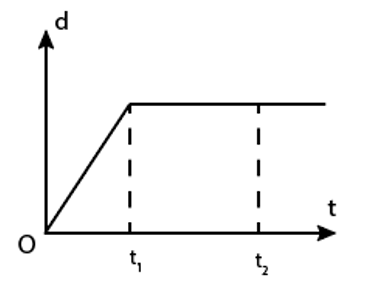
\includegraphics[width=0.25\linewidth]{figs/VN10-2023-PH-TP005-P-4}
	\end{center}
	\choice
	{\True Trong khoảng thời gian từ $0$ đến $t_1$}
	{Trong khoảng thời gian từ $0$ đến $t_2$}
	{Trong khoảng thời gian từ $t_1$ đến $t_2$}
	{Không có lúc nào xe chuyển động thẳng đều}
	\loigiai{}
\end{ex}
% ===================================================================
\begin{ex}
	Phương trình chuyển động của một chất điểm dọc theo trục $Ox$ có dạng: $x = 5 + 60t$ ($x$ đo bằng kilomét và $t$ đo bằng giờ). Chất điểm đó xuất phát từ điểm nào và chuyển động với vận tốc bằng bao nhiêu?
	\choice
	{Từ điểm $O$, với vận tốc $\SI{5}{\kilo\meter/\hour}$}
	{Từ điểm $O$, với vận tốc $\SI{60}{\kilo\meter/\hour}$}
	{Từ điểm cách $O$ $\SI{5}{\kilo\meter/\hour}$, với vận tốc $\SI{5}{\kilo\meter/\hour}$}
	{\True Từ điểm cách $O$ $\SI{5}{\kilo\meter/\hour}$, với vận tốc $\SI{60}{\kilo\meter/\hour}$}
	\loigiai{}
\end{ex}
% ===================================================================
\begin{ex}
Phương trình chuyển động của một chất điểm dọc theo $Ox$ có dạng: $x=5t-12$ (km), với $t$ đo bằng giờ. Độ dịch chuyển của chất điểm từ $\SI{2}{\hour}$ đến $\SI{4}{\hour}$ là	
	\choice
	{$\SI{8}{\kilo\meter}$}
	{$\SI{6}{\kilo\meter}$}
	{\True $\SI{10}{\kilo\meter}$}
	{$\SI{2}{\kilo\meter}$}
	\loigiai{}
\end{ex}
% ===================================================================
\begin{ex}
	Phương trình chuyển động của một chất điểm dọc theo trục $Ox$ có dạng: $x = 4 -10t$ ($x$ đo bằng kilomét và $t$ đo bằng giờ). Quãng đường đi được của chất điểm sau $\SI{2}{\hour}$ chuyển động là
	\choice
	{$\SI{-20}{\kilo\meter}$}
	{\True $\SI{20}{\kilo\meter}$}
	{$\SI{-8}{\kilo\meter}$}
	{$\SI{8}{\kilo\meter}$}
	\loigiai{}
\end{ex}

% ===================================================================
\begin{ex}
	Một xe xuất phát từ lúc 7 giờ 15 phút sáng từ thành phố M, chuyển động thẳng đều tới thành phố N, cách thành phố M $\SI{90}{\kilo\meter}$. Biết tốc độ của xe là $\SI{60}{\kilo\meter/\hour}$, xe đến thành phố N lúc
	\choice
	{9 giờ 45 phút}
	{8 giờ 30 phút}
	{9 giờ 30 phút}
	{\True 8 giờ 45 phút}
	\loigiai{Thời gian để xe đi từ M đến N:
		$$\Delta t=\dfrac{s}{v}=\SI{1.5}{\hour}.$$
		Thời điểm xe đến N:
		$$t=\SI{7}{\hour}\SI{15}{\minute}+\Delta t=\SI{8}{\hour}\SI{45}{\minute}.$$}
\end{ex}
% ===================================================================
\begin{ex}
	Trong nội dung thi đấu môn bơi ếch $\SI{100}{\meter}$, một vận động viên đã hoàn thành đường đua với thành tích $\SI{63.25}{\second}$. Tốc độ trung bình của vận động viên này trong giải thi đấu đó là bao nhiêu?
	\choice
	{\True $\SI{1.58}{\meter/\second}$}
	{$\SI{0.63}{\meter/\second}$}
	{$\SI{6.33}{\meter/\second}$}
	{$\SI{36.75}{\meter/\second}$}
	\loigiai{ Tốc độ trung bình của vận động viên này
		$$v_\text{tb}=\dfrac{s}{t}\approx\SI{1.58}{\meter/\second}.$$}
\end{ex}
% ===================================================================
\begin{ex}
Một ô tô chạy thử nghiệm trên một đoạn đường thẳng. Cứ $\SI{5}{\second}$ thì có một giọt dầu từ động cơ của ô tô rơi thẳng xuống mặt đường. Hình bên cho thấy mô hình các giọt dầu để lại trên mặt đường. Ô tô chuyển động trên đường này với tốc độ trung bình là
\begin{center}
	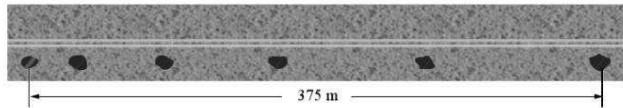
\includegraphics[width=0.5\linewidth]{figs/VN10-2022-PH-TP004-1-P-1}
\end{center}	
	\choice
	{$\SI{12.5}{\meter/\second}$}
	{\True $\SI{15}{\meter/\second}$}
	{$\SI{30}{\meter/\second}$}
	{$\SI{25}{\meter/\second}$}
	\loigiai{Tốc độ trung bình của ô tô:
		$$v_\text{tb}=\dfrac{s}{t}=\dfrac{\SI{375}{\meter}}{\SI{25}{\second}}=\SI{15}{\meter/\second}.$$}
\end{ex}
% ===================================================================
\begin{ex}
	Một xe chuyển động thẳng không đổi chiều, $\SI{1}{\hour}$ đầu xe chạy với tốc độ trung bình $\SI{60}{\kilo\meter/\hour}$ và $\SI{3}{\hour}$ sau xe chạy với tốc độ trung bình $\SI{40}{\kilo\meter/\hour}$. Tốc độ trung bình của xe trong suốt thời gian chuyển động là
	\choice
	{$\SI{48}{\kilo\meter/\hour}$}
	{$\SI{40}{\kilo\meter/\hour}$}
	{$\SI{58}{\kilo\meter/\hour}$}
	{\True $\SI{45}{\kilo\meter/\hour}$}
	\loigiai{$$v_{tb}=\dfrac{v_1t_1+v_2t_2}{t_1+t_2}=\SI{45}{\kilo\meter/\hour}.$$}
\end{ex}
% ===================================================================
\begin{ex}
	Một người đi xe đạp trên $\dfrac{2}{3}$ đoạn đường đầu với tốc độ trung bình $\SI{10}{\kilo\meter/\hour}$ và $\dfrac{1}{3}$ đoạn đường sau với tốc độ trung bình $\SI{20}{\kilo\meter/\hour}$. Tốc độ trung bình của người đi xe đạp trên cả quãng đường là
	\choice
	{\True $\SI{12}{\kilo\meter/\hour}$}
	{$\SI{15}{\kilo\meter/\hour}$}
	{$\SI{17}{\kilo\meter/\hour}$}
	{$\SI{13.3}{\kilo\meter/\hour}$}
	\loigiai{Gọi $s$ là chiều dài đoạn đường
		$$v_{tb}=\dfrac{s}{t_1+t_2}=\dfrac{s}{\dfrac{2s}{3v_1}+\dfrac{s}{3v_2}}=\dfrac{1}{\dfrac{2}{3v_1}+\dfrac{1}{3v_2}}=\SI{12}{\kilo\meter/\hour}.$$}
\end{ex}
% ===================================================================
\begin{ex}
	Hình vẽ bên là đồ thị độ dịch chuyển - thời gian của một chiếc xe ô tô chạy từ $A$ đến $B$ trên một đường thẳng. Vận tốc của xe bằng
\begin{center}
	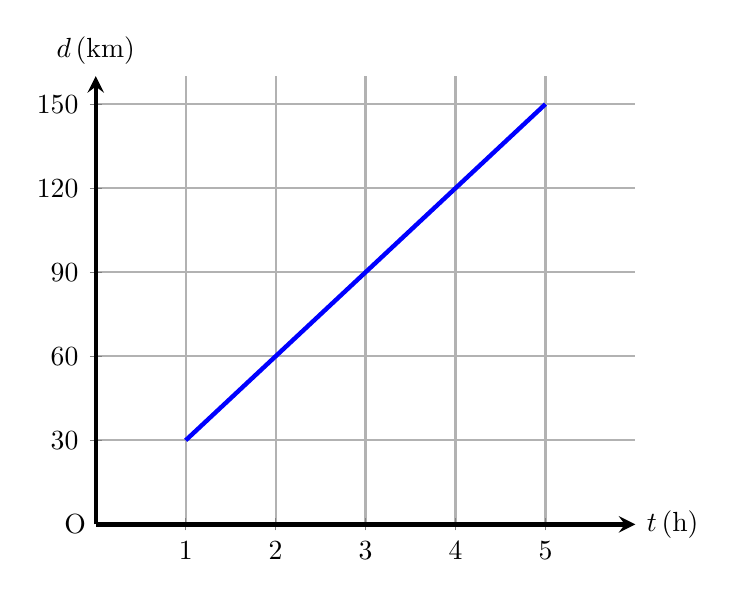
\begin{tikzpicture}  
		\begin{axis}[  ultra thick,
			xmin=0,  
			xmax=6,  
			xtick={0,1,...,5},
			ytick={0,30,...,150},
			minor x tick num=0,
			minor y tick num=0,
			ymin=0,  
			ymax=160, 
			samples=300,
			axis lines=center, 
			grid style={step=1, line width =0.4pt, color=gray!30!white},
			grid=both,
			major grid style={line width=0.8pt,gray!60!white},
			xlabel=$\xsi{t}{\left(\si{\hour}\right)}$, 		ylabel=$\xsi{d}{\left(\si{\kilo\meter}\right)}$,
			every axis y label/.style={at=(current axis.above origin),anchor=south},  
			every axis x label/.style={at=(current axis.right of origin),anchor=west},  ]
			\addplot [ultra thick, blue, smooth, domain=1:5] {30*x};			 
		\end{axis}  
		\node[left] at (0,0) {O};
	\end{tikzpicture}
\end{center}
	\choice
	{\True $\SI{30}{\kilo\meter/\hour}$}
	{$\SI{150}{\kilo\meter/\hour}$}
	{$\SI{120}{\kilo\meter/\hour}$}
	{$\SI{100}{\kilo\meter/\hour}$}
	\loigiai{}
\end{ex}
% ===================================================================
\begin{ex}
Một chất điểm chuyển động trên một đường thẳng. Đồ thị độ dịch chuyển theo thời gian của chất điểm được mô tả như hình vẽ. Tốc độ trung bình của chất điểm trong khoảng thời gian từ 0 đến $\SI{5}{\second}$ là
	\begin{center}
		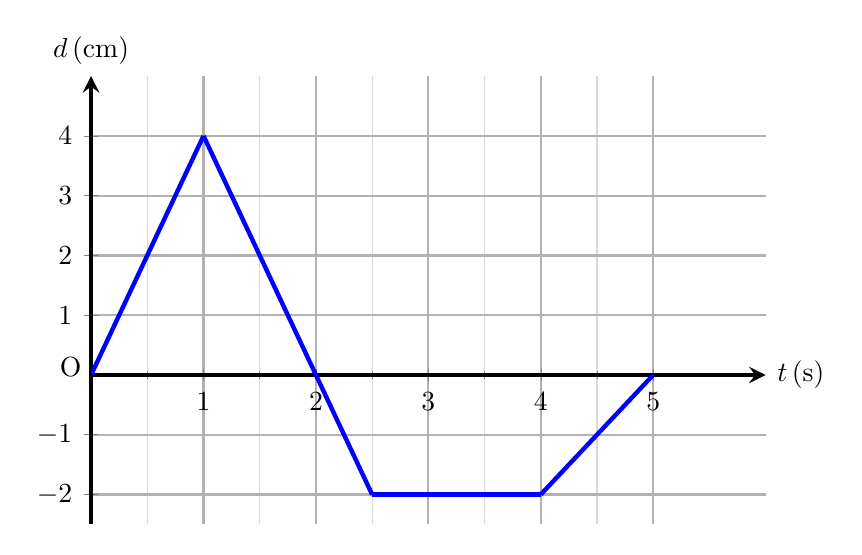
\begin{tikzpicture}  
			\begin{axis}[  ultra thick,xscale=1.25,
				xmin=0,  
				xmax=6,  
				xtick={0,1,...,5},
				ytick={-2,-1,0,1,...,4},
				minor x tick num=1,
				minor y tick num=0,
				ymin=-2.5,  
				ymax=5, 
				samples=300,
				axis lines=center, 
				grid style={step=1, line width =0.4pt, color=gray!30!white},
				grid=both,
				major grid style={line width=0.8pt,gray!60!white},
				xlabel=$\xsi{t}{\left(\si{\second}\right)}$, 		ylabel=$\xsi{d}{\left(\si{\centi\meter}\right)}$,
				every axis y label/.style={at=(current axis.above origin),anchor=south},  
				every axis x label/.style={at=(current axis.right of origin),anchor=west},  ]
				\addplot [ultra thick, blue, smooth, domain=0:1] {4*x};	
				\addplot [ultra thick, blue, smooth, domain=1:2.5] {4-4*(x-1)};		
				\addplot [ultra thick, blue, smooth, domain=2.5:4] {-2};	 
				\addplot [ultra thick, blue, smooth, domain=4:5] {-2+2*(x-4)};
				
			\end{axis}  
		\node[left] at (0,2) {O};
			
		\end{tikzpicture}
	\end{center}
	\choice
	{$\SI{1.6}{\centi\meter/\second}$}
	{$\SI{6.4}{\centi\meter/\second}$}
	{$\SI{4.8}{\centi\meter/\second}$}
	{\True $\SI{2.4}{\centi\meter/\second}$}
	\loigiai{
Tốc độ trung bình của chất điểm:
$$v_\text{tb}=\dfrac{s}{t}=\dfrac{4+4+2+2}{5}=\SI{2.4}{\centi\meter/\second}.$$	
}
\end{ex}
% ===================================================================
\begin{ex}
	Đồ thị toạ độ - thời gian của hai xe (I) và (II) cùng chuyển động trên một đường thẳng được thể hiện như hình bên. Thời điểm hai xe gặp nhau là
	\begin{center}
		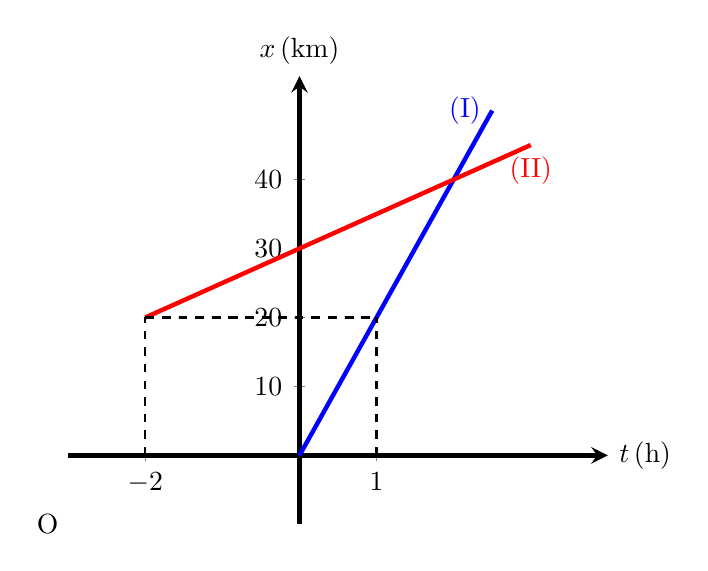
\begin{tikzpicture}  
			\begin{axis}[  ultra thick,
				xmin=-3,  
				xmax=4,  
				xtick={-2,0,1},
				ytick={0,10,...,40},
				minor x tick num=0,
				minor y tick num=0,
				ymin=-10,  
				ymax=55, 
				samples=300,
				axis lines=center, 
%				grid style={step=1, line width =0.4pt, color=gray!30!white},
%				grid=both,
%				major grid style={line width=0.8pt,gray!60!white},
				xlabel=$\xsi{t}{\left(\si{\hour}\right)}$, 		ylabel=$\xsi{x}{\left(\si{\kilo\meter}\right)}$,
				every axis y label/.style={at=(current axis.above origin),anchor=south},  
				every axis x label/.style={at=(current axis.right of origin),anchor=west},  ]
				\addplot [ultra thick, blue, smooth, domain=0:2.5] {20*x} node[left] {(I)};	
				\addplot [ultra thick, red, smooth, domain=-2:3] {30+5*x} node[below] {(II)};	
				\addplot [thick, dashed, domain=-2:1] {20} ;	
				\draw[thick, dashed] (axis cs:-2,0) --(-2,20);	 
				\draw[thick, dashed] (axis cs:1,0) --(1,20);
			\end{axis}  
			\node[left] at (0,0) {O};
		\end{tikzpicture}
	\end{center}
	\choice
	{$\SI{1}{\hour}$}
	{\True$\SI{2}{\hour}$}
	{$\SI{2.5}{\hour}$}
	{$\SI{1.33}{\hour}$}
	\loigiai{}
\end{ex}

% ===================================================================
\begin{ex}
	Hình dưới là đồ thị độ dịch chuyển - thời gian của hai vật chuyển động thẳng cùng hướng. Tỉ lệ vận tốc $\dfrac{v_A}{v_B}$ là
	\begin{center}
		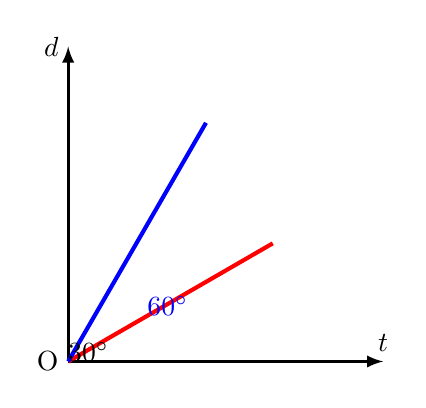
\begin{tikzpicture} 
			\coordinate (O)  at (0,0);
			\coordinate (t) at (4,0);
			\coordinate (d) at (0,4);
			\coordinate (A) at ($(O)+(30:3)$);
			\coordinate (B) at ($(O)+(60:3.5)$);
			\draw[line width=1pt, -latex] (O)--(d);
			\draw[line width=1pt, -latex] (O)--(t);
			\draw[line width=1.5pt, red] (O)--(A);
			\draw[line width=1.5pt, blue] (O)--(B);
			\node[left] at (O) {O};
			\node[above] at (t) {$t$};
			\node[left] at (d) {$d$};
			\tkzFillAngle[size=0.75cm,color=red, fill=red, opacity=0.25](t,O,A);
			\tkzLabelAngle[color=red,pos=1.2](t,O,A){$\SI{30}{\degree}$}
				\tkzMarkAngle[size=0.5cm,color=blue](t,O,B);
		\node[blue] at (0.75,0.7) {$\SI{60}{\degree}$};
		\end{tikzpicture}
	\end{center}
	\choice
	{$\dfrac{3}{1}$}
	{$\dfrac{1}{3}$}
	{$\dfrac{\sqrt{3}}{1}$}
	{$\dfrac{1}{\sqrt{3}}$}
	\loigiai{}
\end{ex}


\Closesolutionfile{ans}
\begin{center}
	\textbf{--- HẾT ---}
\end{center}
%\tikzstyle{startstop} = [rectangle, rounded corners, minimum width=10cm, minimum height=1.5cm,text centered, draw=black, fill=green!20]
\begin{center}
	\begin{tikzpicture}
		\node (start) [startstop] {\bfseries \text{ÔN TẬP: GIA TỐC - CHUYỂN ĐỘNG THẲNG BIẾN ĐỔI ĐỀU}};
	\end{tikzpicture}
\end{center}
\setcounter{section}{0}
\Opensolutionfile{ans}[ans/G10TUAN4-TN]
% ===================================================================
\begin{ex}
	Gia tốc là đại lượng
	\choice
	{vô hướng, đặc trưng cho sự biến thiên nhanh hay chậm của chuyển động}
	{vô hướng, đặc trưng cho tính không đổi của vận tốc}
	{vector, đặc trưng cho sự biến thiên nhanh hay chậm của chuyển động}
	{\True vector, đặc trưng cho sự biến thiên nhanh hay chậm của vận tốc}
	\loigiai{}
\end{ex}
% ===================================================================
\begin{ex}
	Chọn ý \textbf{sai}. Chuyển động thẳng nhanh dần đều có
	\choice
	{\True vector gia tốc ngược chiều vector vận tốc}
	{vận tốc tức thời là hàm số bậc nhất theo thời gian}
	{toạ độ là hàm số bậc hai theo thời gian}
	{gia tốc không đổi theo thời gian}
	\loigiai{}
\end{ex}
% ===================================================================
\begin{ex}
	Một xe máy đang đứng yên, sau đó khởi động và bắt đầu tăng tốc. Nếu chọn chiều dương cùng chiều chuyển động của xe, nhận xét nào sau đây là \textbf{đúng}? 
	\choice
	{$a<0$, $v<0$}
	{$a>0$, $v<0$}
	{\True $a>0$, $v>0$}
	{$a<0$, $v>0$}
	\loigiai{}
\end{ex}

% ===================================================================
\begin{ex}
Công thức tính quãng đường đi được của vật chuyển động thẳng nhanh dần đều là	
	\choice
	{\True $s=v_0t+\frac{1}{2}at^2$ ($a$ và $v_0$ cùng dấu)}
	{$s=v_0t+\frac{1}{2}at^2$ ($a$ và $v_0$ trái dấu)}
	{$s=at+\frac{1}{2}v_0t^2$ ($a$ và $v_0$ cùng dấu)}
	{$s=at+\frac{1}{2}v_0t^2$ ($a$ và $v_0$ trái dấu)}
	\loigiai{}
\end{ex}
% ===================================================================
\begin{ex}
Tàu hoả đang chuyển động thẳng với tốc độ $\SI{60}{\kilo\meter/\hour}$ thì bị hãm phanh, chuyển động chậm dần đều. Sau khi đi thêm được $\SI{450}{\meter}$ thì tốc độ của tàu chỉ còn $\SI{15}{\kilo\meter/\hour}$. Quãng đường tàu còn đi thêm được đến khi dừng hẳn là	
	\choice
	{$\SI{60}{\meter}$}
	{$\SI{45}{\meter}$}
	{$\SI{15}{\meter}$}
	{\True $\SI{30}{\meter}$}
	\loigiai{}
\end{ex}
% ===================================================================
\begin{ex}
Một ô tô chuyển động chậm dần đều. Sau $\SI{10}{\second}$, tốc độ của ô tô giảm từ $\SI{6}{\meter/\second}$ còn $\SI{4}{\meter/\second}$. Quãng đường ô tô đi được trong khoảng thời gian $\SI{10}{\second}$ đó là	
	\choice
	{$\SI{70}{\meter}$}
	{$\SI{50}{\meter}$}
	{$\SI{40}{\meter}$}
	{\True $\SI{100}{\meter}$}
	\loigiai{}
\end{ex}
% ===================================================================
\begin{ex}
Một ô tô đang chuyển động với tốc độ $\SI{10}{\meter/\second}$ thì bắt đầu tăng tốc, chuyển động nhanh dần đều. Sau $\SI{20}{\second}$ kể từ khi tăng tốc, ô tô đạt tốc độ $\SI{14}{\meter/\second}$. Sau $\SI{50}{\second}$ kể từ lúc tăng tốc, gia tốc và vận tốc của ô tô lần lượt là	
	\choice
	{$\SI{0.2}{\meter/\second^2}$ và $\SI{18}{\meter/\second}$}
	{\True $\SI{0.2}{\meter/\second^2}$ và $\SI{20}{\meter/\second}$}
	{$\SI{0.4}{\meter/\second^2}$ và $\SI{38}{\meter/\second}$}
	{$\SI{0.1}{\meter/\second^2}$ và $\SI{28}{\meter/\second}$}
	\loigiai{}
\end{ex}
% ===================================================================
\begin{ex}
	Một vật chuyển động thẳng có quãng đường đi trong một giai đoạn phụ thuộc thời gian dạng $s=-t^2+3t$ ($s$ đo bằng $\si{\meter}$; $t$ đo bằng giây). Biểu thức vận tốc của vật theo thời gian trong giai đoạn này được xác định bởi
	\choice
	{$v=3+2t$}
	{$v=2-3t$}
	{$v=3-t$}
	{\True $v=3-2t$}
	\loigiai{}
\end{ex}

% ===================================================================
\begin{ex}
Một xe chuyển động trên đường thẳng với biểu thức toạ độ phụ thuộc thời gian: $x=0,4t^2+2t+1$ ($x$ tính bằng $\si{\meter}$; $t$ tính bằng $\si{\second}$). Vận tốc của xe tại thời điểm $t=\SI{5}{\second}$ là
	\choice
	{$\SI{10.4}{\meter/\second}$}
	{$\SI{4.0}{\meter/\second}$}
	{$\SI{5.0}{\meter/\second}$}
	{\True $\SI{6.0}{\meter/\second}$}
	\loigiai{}
\end{ex}

% ===================================================================
\begin{ex}
Một ô tô đang chạy với tốc độ $\SI{10}{\meter/\second}$ trên đoạn đường thẳng thì người lái xe tăng ga và ô tô chuyển động nhanh dần đều. Sau một khoảng thời gian, ô tô đạt tốc độ $\SI{15}{\meter/\second}$. Tốc độ trung bình của ô tô trong khoảng thời gian đó là	
	\choice
	{\True $\SI{12.5}{\meter/\second}$}
	{$\SI{9.5}{\meter/\second}$}
	{$\SI{21}{\meter/\second}$}
	{$\SI{2.5}{\meter/\second}$}
	\loigiai{}
\end{ex}
% ===================================================================
\begin{ex}
	Một vật chuyển động thẳng có phương trình toạ độ $x=20t^2+40t+6$ ($\si{\centi\meter}$; $\si{\second}$). Gia tốc và tính chất chuyển động của vật là
	\choice
	{\True $\SI{40}{\centi\meter/\second^2}$; vật chuyển động nhanh dần đều}
	{$\SI{40}{\centi\meter/\second^2}$; vật chuyển động chậm dần đều}
	{$\SI{20}{\centi\meter/\second^2}$; vật chuyển động nhanh dần đều}
	{$\SI{20}{\centi\meter/\second^2}$; vật chuyển động chậm dần đều}
	\loigiai{}
\end{ex}
% ===================================================================
\begin{ex}
	Lúc $\SI{1}{\hour}$, một xe máy qua A với tốc độ $\SI{10}{\meter/\second}$, chuyển động nhanh dần đều với gia tốc $\SI{1}{\meter/\second^2}$ đuổi theo một xe đạp đang chuyển động nhanh dần đều qua B với tốc độ đầu là $\SI{2}{\meter/\second}$ và với gia tốc $\SI{0.5}{\meter/\second^2}$. Sau $\SI{20}{\second}$ thì xe máy đuổi kịp xe đạp. Khoảng cách AB là
	\choice
	{$\SI{360}{\meter}$}
	{$\SI{160}{\meter}$}
	{$\SI{165}{\meter}$}
	{\True $\SI{260}{\meter}$}
	\loigiai{}
\end{ex}
% ===================================================================
\begin{ex}
	Hai người đi xe đạp khởi hành cùng 1 lúc và đi ngược chiều nhau. Người thứ nhất có tốc độ đầu là $\SI{18}{\kilo\meter/\hour}$ và chuyển động chậm dần đều với gia tốc có độ lớn $\SI{20}{\centi\meter/\second^2}$. Người thứ 2 có tốc độ đầu là $\SI{5.4}{\kilo\meter/\hour}$ và chuyển động nhanh dần đều với gia tốc có độ lớn $\SI{0.2}{\meter/\second^2}$. Khoảng cách ban đầu giữa hai người là $\SI{130}{\meter}$. Sau bao lâu 2 người sẽ gặp nhau và gặp nhau ở vị trí nào?
	\choice
	{\True Sau $\SI{20}{\second}$, cách A đoạn $\SI{60}{\kilo\meter}$}
	{Sau $\SI{17.5}{\second}$, cách A đoạn $\SI{56.9}{\kilo\meter}$}
	{Sau $\SI{20}{\second}$, cách B đoạn $\SI{60}{\kilo\meter}$}
	{Sau $\SI{17.5}{\second}$, cách B đoạn $\SI{56.9}{\kilo\meter}$}
	\loigiai{}
\end{ex}
% ===================================================================
\begin{ex}
	Một vật chuyển động trên đường thẳng có đồ thị vận tốc - thời gian như hình vẽ. Quãng đường vật đi được trong $\SI{400}{\second}$ là 
	\begin{center}
		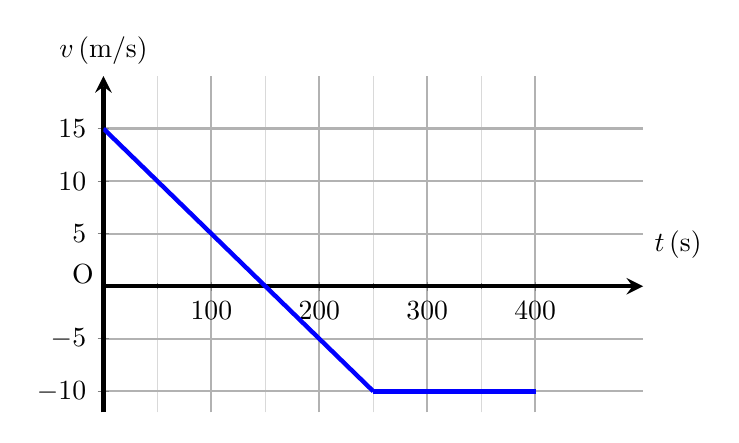
\begin{tikzpicture}  
			\begin{axis}[  ultra thick,yscale=0.75,
				xmin=0,  
				xmax=500,  
				xtick={0,100,...,400},
				ytick={-10,-5,...,15},
				minor x tick num=1,
				minor y tick num=0,
				ymin=-12,  
				ymax=20, 
				samples=300,
				axis lines=center, 
				grid style={step=1, line width =0.4pt, color=gray!30!white},
				grid=both,
				major grid style={line width=0.8pt,gray!60!white},
				xlabel=$\xsi{t}{\left(\si{\second}\right)}$, 		ylabel=$\xsi{v}{\left(\si{\meter/\second}\right)}$,
				every axis y label/.style={at=(current axis.above origin),anchor=south},  
				every axis x label/.style={at=(current axis.right of origin),anchor=west},  ]
				\addplot [ultra thick, blue, smooth, domain=0:250] {15-0.1*x};  
				\addplot [ultra thick, blue, smooth, domain=250:400] {-10};
			 
			\end{axis}  
			\node[below left] at (0,2) {O};
		\end{tikzpicture}
	\end{center}
	\choice
	{$\SI{4625}{\meter}$}
	{\True $\SI{3125}{\meter}$}
	{$\SI{4250}{\meter}$}
	{$\SI{2625}{\meter}$}
	\loigiai{}
\end{ex}
% ===================================================================
\begin{ex}
Một vật chuyển động thẳng có đồ thị vận tốc theo thời gian như hình vẽ. Quãng đường vật đi được trong giai đoạn chuyển động chậm dần đều là	
\begin{center}
	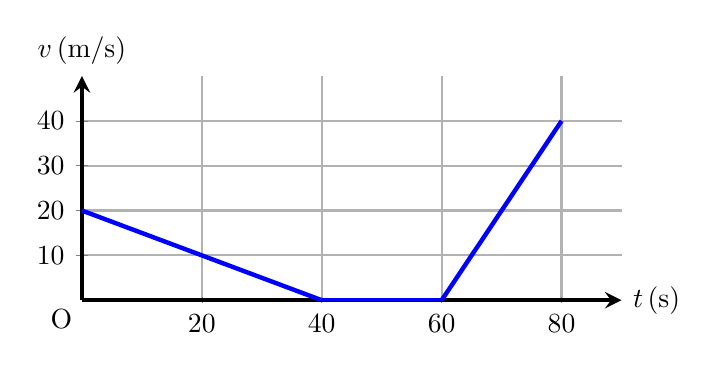
\begin{tikzpicture}  
		\begin{axis}[  ultra thick,yscale=0.5,
			xmin=0,  
			xmax=90,  
			xtick={0,20,...,80},
			ytick={0,10,...,40},
			minor x tick num=0,
			minor y tick num=0,
			ymin=0,  
			ymax=50, 
			samples=300,
			axis lines=center, 
			grid style={step=1, line width =0.4pt, color=gray!30!white},
			grid=both,
			major grid style={line width=0.8pt,gray!60!white},
			xlabel=$\xsi{t}{\left(\si{\second}\right)}$, 		ylabel=$\xsi{v}{\left(\si{\meter/\second}\right)}$,
			every axis y label/.style={at=(current axis.above origin),anchor=south},  
			every axis x label/.style={at=(current axis.right of origin),anchor=west},  ]
			\addplot [ultra thick, blue, smooth, domain=0:40] {20-0.5*x};  
			\addplot [ultra thick, blue, smooth, domain=40:60] {0};
			\addplot [ultra thick, blue, smooth, domain=60:80] {2*(x-60)};
			
		\end{axis}  
	\node[below left] at (0,0) {O}; 
	\end{tikzpicture}
\end{center}
	\choice
	{$\SI{600}{\meter}$}
	{$\SI{800}{\meter}$}
	{$\SI{200}{\meter}$}
	{\True $\SI{400}{\meter}$}
	\loigiai{}
\end{ex}







\Closesolutionfile{ans}
\begin{center}
	\textbf{--- HẾT ---}
\end{center}
%\setcounter{section}{0}
\begin{center}
	\textbf{\large BẢNG ĐÁP ÁN}
\end{center}
\section{}
\inputansbox{10}{ans/G10C1TN}
\section{}
\inputansbox[2]{2}{ans/G10C1TF}
\section{}
\inputansbox[3]{6}{ans/G10C1TL}\newpage
\tikzstyle{startstop} = [rectangle, rounded corners, minimum width=10cm, minimum height=1.5cm,text centered, draw=black, fill=green!20]
\begin{center}
	\begin{tikzpicture}
		\node (start) [startstop] {\bfseries \text{ÔN TẬP: CHƯƠNG MỞ ĐẦU}};
	\end{tikzpicture}
\end{center}
\section{Câu trắc nghiệm nhiều phương án lựa chọn}
\textit{Thí sinh trả lời từ câu 1 đến câu 24. Mỗi câu hỏi thí sinh chọn một phương án}
\setcounter{ex}{0}
\Opensolutionfile{ans}[ans/G10C1TN]
% ===================================================================
\begin{ex}
	Đối tượng nghiên cứu của vật lí là gì?
	\choice
	{Các dạng vận động và tương tác của vật chất}
	{Quy luật tương tác của các dạng năng lượng}
	{\True Các dạng vận động của vật chất và năng lượng}
	{Quy luật vận động, phát triển của sự vật - hiện tượng}
	\loigiai{}
\end{ex}
% ===================================================================
\begin{ex}
Lĩnh vực nghiên cứu nào sau đây là của vật lí?	
	\choice
	{Nghiên cứu về sự thay đổi của các chất khi kết hợp với nhau}
	{Nghiên cứu sự phát triển của vi khuẩn}
	{Nghiên cứu về sự hình thành và phát triển của các tầng lớp, giai cấp trong xã hội}
	{\True Nghiên cứu về các dạng chuyển động và các dạng năng lượng khác nhau}
	\loigiai{}
\end{ex}
% ===================================================================
\begin{ex}
	Thành tựu nghiên cứu nào sau đây của Vật lí được coi là có vai trò quan trọng trong việc mở đầu cho cuộc cách mạng công nghệ lần thứ nhất?
	\choice
	{Nghiên cứu về lực vạn vật hấp dẫn}
	{\True Nghiên cứu về nhiệt động lực học}
	{Nghiên cứu về cảm ứng điện từ}
	{Nghiên cứu về thuyết tương đối}
	\loigiai{}
\end{ex}
% ===================================================================
\begin{ex}
	Trong các hoạt động dưới đây, hoạt động nào tuân thủ nguyên tắc an toàn khi sử dụng điện?
	\choice
	{Sửa chữa điện khi chưa ngắt nguồn điện}
	{Chạm tay trực tiếp vào ổ điện, dây điện trần hoặc dây dẫn điện bị hở}
	{Đến gần nhưng không tiếp xúc với các máy biến thế và lưới điện cao áp}
	{\True Kiểm tra mạch có điện bằng bút thử điện}
	\loigiai{}
\end{ex}
% ===================================================================
\begin{ex}
	Trong các hoạt động dưới đây, hoạt động nào tuân thủ nguyên tắc an toàn khi làm việc với các nguồn phóng xạ?
	\choice
	{Ăn uống, trang điểm trong phòng làm việc có chứa chất phóng xạ}
	{\True Sử dụng phương tiện phòng hộ cá nhân như quần áo phòng hộ, mũ, găng tay, áo chì, \dots}
	{Đổ rác thải phóng xạ tại các khu tập trung rác thải sinh hoạt}
	{Dùng hộp chứa bằng vật liệu thuỷ tinh để đựng chất phóng xạ}
	
	\loigiai{}
\end{ex}
% ===================================================================
\begin{ex}
	Công nghệ chất bán dẫn liên tục phá vỡ các rào cản để có thể tạo ra những con chip nhỏ hơn, nhanh hơn, mạnh hơn và tiết kiệm điện năng hơn. Vừa mới đây, IBM tuyên bố đã tạo ra một con chip $\SI{2}{\nano\meter}$.	Trong khi đó, kích thước trung bình của một gạo là $\SI{6}{\milli\meter}$. So với hạt gạo, con chip trên nhỏ hơn khoảng bao nhiêu lần?
	\begin{center}
		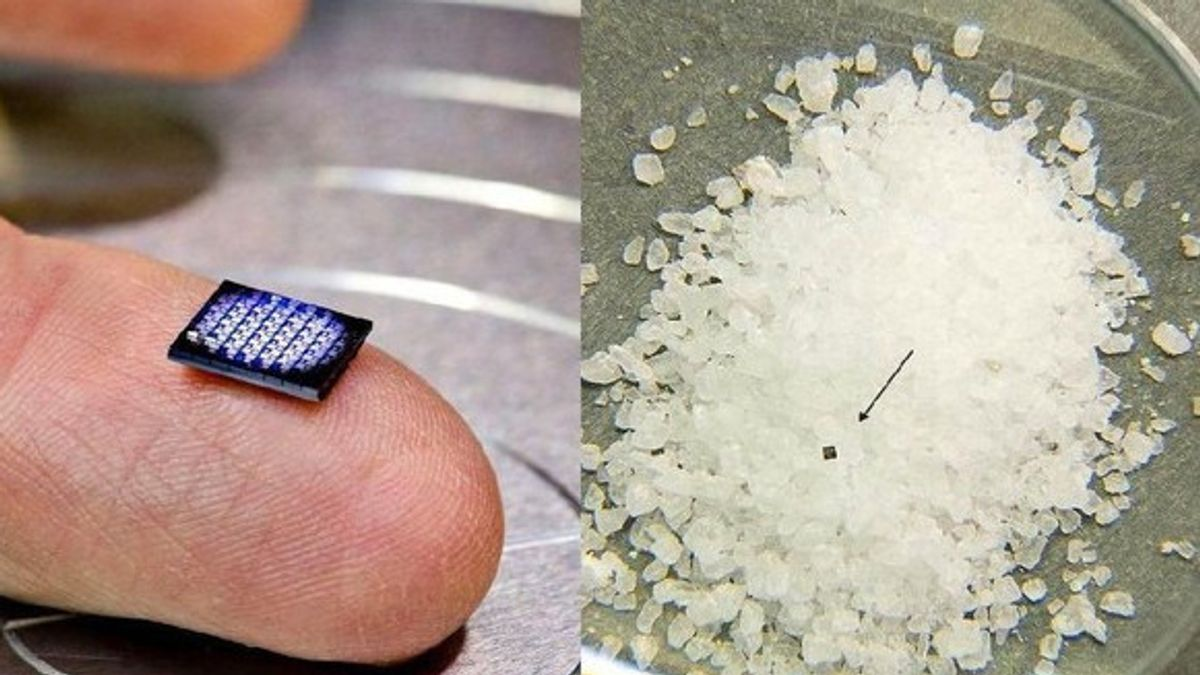
\includegraphics[width=0.4\linewidth]{figs/G10-CHUONG1-6}
		\captionof{figure}{So sánh kích thước chip $\SI{2}{\nano\meter}$ của IBM với các hạt gạo vỡ}
	\end{center}
	\choice
	{$3\cdot10^9$ lần}
	{\True $3\cdot10^6$ lần}
	{$3000$ lần}
	{$0,003$ lần}
	\loigiai{}
\end{ex}
% ===================================================================
\begin{ex}
	Chọn đáp án có từ /cụm từ thích hợp để hoàn thành bảng sau:
	\begin{center}
		\begin{tabular}{|c|c|c|}
			\hline
			\thead{Đơn vị} & \thead{Kí hiệu} & \thead{Đại lượng }\\
			\hline
			kelvin & (1) & (2)\\
			\hline
			ampe & $\si{\ampere}$ & (3)\\
			\hline
			candela & $\si{\candela}$ & (4)\\
			\hline
		\end{tabular}
	\end{center}
	\choice
	{(1) $\si{\kelvin}$; (2) Khối lượng; (3) Cường độ dòng điện; (4) Lượng chất}
	{\True (1) $\si{\kelvin}$; (2) Nhiệt độ; (3) Cường độ dòng điện; (4) Cường độ ánh sáng}
	{(1) $\si{\kelvin}$; (2) Nhiệt độ; (3) Cường độ dòng điện; (4) Lượng chất}
	{(1) $\si{\kelvin}$; (2) Khối lượng; (3) Cường độ dòng điện; (4) Cường độ ánh sáng}
	\loigiai{}
\end{ex}
% ===================================================================
\begin{ex}
	Đơn vị nào sau đây không thuộc thứ nguyên $L$ [Chiều dài]?
	\choice
	{Dặm}
	{Hải lí}
	{Năm ánh sáng}
	{\True Lạng}
	\loigiai{}
\end{ex}
% ===================================================================
\begin{ex}
	Chọn đáp án có từ/cụm từ thích hợp để hoàn thành các câu sau:
	\begin{itemize}
		\item[-] Các số hạng trong phép cộng (hoặc trừ) phải có cùng (1) \dots và nên chuyển về cùng (2) \dots.
		\item[-] (3) \dots của một biểu thức vật lí phải có cùng thứ nguyên.
	\end{itemize}
	\choice
	{(1) đơn vị; (2) thứ nguyên; (3)  Đại lượng}
	{(1) thứ nguyên; (2) đại lượng; (3) Hai vế}
	{(1) đơn vị; (2) đại lượng; (3) Hai vế}
	{\True (1) thứ nguyên; (2) đơn vị; (3) Hai vế}
	\loigiai{}
\end{ex}
% ===================================================================
\begin{ex}
	Trong các phép đo dưới đây, đâu là phép đo trực tiếp?
	\begin{enumerate}[label=(\arabic*)]
		\item Dùng thước đo chiều cao.
		\item Dùng cân đo cân nặng.
		\item Dùng cân và ca đong đo khối lượng riêng của nước.
		\item Dùng đồng hồ và cột cây số đo tốc độ của người lái xe.
	\end{enumerate}
	\choice
	{\True (1), (2)}
	{(1), (2), (4)}
	{(2), (3), (4)}
	{(2), (4)}
	\loigiai{}
\end{ex}
% ===================================================================
\begin{ex}
	Đáp án nào sau đây có 1 đơn vị cơ bản và 1 đơn vị dẫn xuất?
	\choice
	{mét, kilogram}
	{pascal, joule}
	{candela, kelvin}
	{\True newton, mol}
	\loigiai{}
\end{ex}


% ===================================================================
\begin{ex}
		Đại lượng đặc trưng cho tính chất nhanh hay chậm của chuyển động là 
	\choice
	{toạ độ}
	{gia tốc}
	{quãng đường đi}
	{\True tốc độ}
	\loigiai{}
\end{ex}
% ===================================================================
\begin{ex}
	Khi nhìn vào tốc kế của ô tô đang chạy, số chỉ trên tốc kế cho ta biết
	\choice
	{gia tốc tức thời của ô tô}
	{vận tốc tức thời của ô tô}
	{\True tốc độ tức thời của ô tô}
	{tốc độ trung bình của ô tô}
	\loigiai{}
\end{ex}
% ===================================================================
\begin{ex}
	Đâu là cách viết kết quả đo \textbf{đúng}?
	\choice
	{$A=\overline{A}+\Delta A$}
	{$A=\overline{A}-\Delta A$}
	{\True $A=\overline{A}\pm\Delta A$}
	{$A=\overline{A}:\Delta A$}
	\loigiai{}
\end{ex}

% ===================================================================
\begin{ex}
	Giá trị nào sau đây có 2 chữ số có nghĩa (CSCN)?
	\choice
	{\True $\SI{210}{\meter}$}
	{$\SI{20}{\meter}$}
	{$\SI{0.02}{\meter}$}
	{$\SI{201}{\meter}$}
	\loigiai{}
\end{ex}
% ===================================================================
\begin{ex}
Sai số tương đối của đại lượng $A$ được tính bởi công thức	
	\choice
	{\True $\delta A=\dfrac{\Delta A}{\overline{A}}\cdot\SI{100}{\percent}$}
	{$\overline{\Delta A}=\dfrac{\Delta A_1+\Delta A_2+\dots+\Delta A_n}{n}$}
	{$A=\overline{A}\pm\Delta A$}
	{$\delta A=\dfrac{\overline{A}}{\Delta A}$}
	\loigiai{}
\end{ex}

% ===================================================================
\begin{ex}
Một học sinh dùng thước đo chiều dài của chiếc bút chì như hình bên dưới. Nếu lấy sai số dụng cụ bằng 1 nửa độ chia nhỏ nhất thì sai số hệ thống trong phép đo trên là	
\begin{center}
	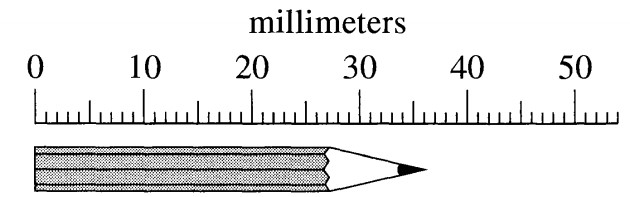
\includegraphics[width=0.4\linewidth]{../figs/G10-CHUONG1-1}
\end{center}
	\choice
	{$\SI{1}{\milli\meter}$}
	{\True $\SI{0.5}{\milli\meter}$}
	{$\SI{1}{\centi\meter}$}
	{$\SI{0.5}{\milli\meter}$}
	\loigiai{}
\end{ex}

% ===================================================================
\begin{ex}
	Một bánh xe có bán kính $R=\xsi{10\pm0,5}{\centi\meter}$. Sai số tương đối của chu vi bánh xe là
	\choice
	{$\SI{0.05}{\percent}$}
	{\True $\SI{5}{\percent}$}
	{$\SI{10}{\percent}$}
	{$\SI{25}{\percent}$}
	\loigiai{
$$\delta R=\dfrac{\Delta R}{\overline{R}}\cdot\SI{100}{\percent}=\SI{5}{\percent}.$$	
}
\end{ex}
% ===================================================================
\begin{ex}
	Thứ nguyên của vận tốc là
	\choice
	{$LT$}
	{$L^{-1}T$}
	{$L^{-1}T^{-1}$}
	{\True $LT^{-1}$}
	\loigiai{
\begin{eqnarray*}
	v&=&\dfrac{s}{t}\\
	\Rightarrow \left[v\right]&=&\dfrac{\left[s\right]}{\left[t\right]}=LT^{-1}.
\end{eqnarray*}	
}
\end{ex}
% ===================================================================
\begin{ex}
	Cho thứ nguyên của trọng lượng là $MLT^{-2}$. Thứ nguyên của trọng lượng riêng là
	\choice
	{$MLT^{-1}$}
	{$MLT^{-2}$}
	{$ML^{-2}T^{-1}$}
	{\True $ML^{-2}T^{-2}$}
	\loigiai{
\begin{eqnarray*}
	d&=&\dfrac{P}{V}\\
	\Rightarrow \left[d\right]&=&\dfrac{\left[P\right]}{\left[V\right]}\\
	\Leftrightarrow \left[d\right]&=&\dfrac{MLT^{-2}}{L^3}=ML^{-2}T^{-2}.
\end{eqnarray*}	
}
\end{ex}
% ===================================================================
\begin{ex}
Một xe xuất phát từ lúc 7 giờ 15 phút sáng từ thành phố M, chuyển động thẳng đều tới thành phố N, cách thành phố M $\SI{90}{\kilo\meter}$. Biết tốc độ của xe là $\SI{60}{\kilo\meter/\hour}$, xe đến thành phố N lúc	
	\choice
	{9 giờ 45 phút}
	{8 giờ 30 phút}
	{9 giờ 30 phút}
	{\True 8 giờ 45 phút}
	\loigiai{
Thời gian để xe đi từ M đến N:
$$\Delta t=\dfrac{s}{v}=\SI{1.5}{\hour}.$$
Thời điểm xe đến N:
$$t=\SI{7}{\hour}\SI{15}{\minute}+\Delta t=\SI{8}{\hour}\SI{45}{\minute}.$$	
}
\end{ex}
% ===================================================================
\begin{ex}
	Một vận động viên chạy cự li $\SI{600}{\meter}$ mất $\SI{74.75}{\second}$. Tốc độ trung bình của vận động viên đó là
	\choice
	{\True $\SI{8.03}{\meter/\second}$}
	{$\SI{9.03}{\meter/\second}$}
	{$\SI{10.03}{\meter/\second}$}
	{$\SI{11.03}{\meter/\second}$}
	\loigiai{
Tốc độ trung bình của vận động viên:
$$v_\text{tb}=\dfrac{s}{\Delta t}=\SI{8.03}{\meter/\second}.$$	
}
\end{ex}
% ===================================================================
\begin{ex}
	Một người bơi dọc theo chiều dài $\SI{55}{\meter}$ của bể bơi hết $\SI{50}{\second}$ rồi quay về lại chỗ xuất phát trong $\SI{60}{\second}$. Trong suốt quãng đường đi và về vận tốc trung bình của người đó là
	\choice
	{\True $\SI{0}{\meter/\second}$}
	{$\SI{1.0}{\meter/\second}$}
	{$\SI{1.1}{\meter/\second}$}
	{$\SI{2.0}{\meter/\second}$}
	\loigiai{
Vì điểm đầu của quĩ đạo chuyển động trùng với điểm cuối nên $d=0\Rightarrow v=0$.	
}
\end{ex}

% ===================================================================
\begin{ex}
	Hình bên là đồ thị toạ độ - thời gian của một chiếc xe máy đang chạy trên đường thẳng. Xe này có tốc độ là
	\begin{center}
		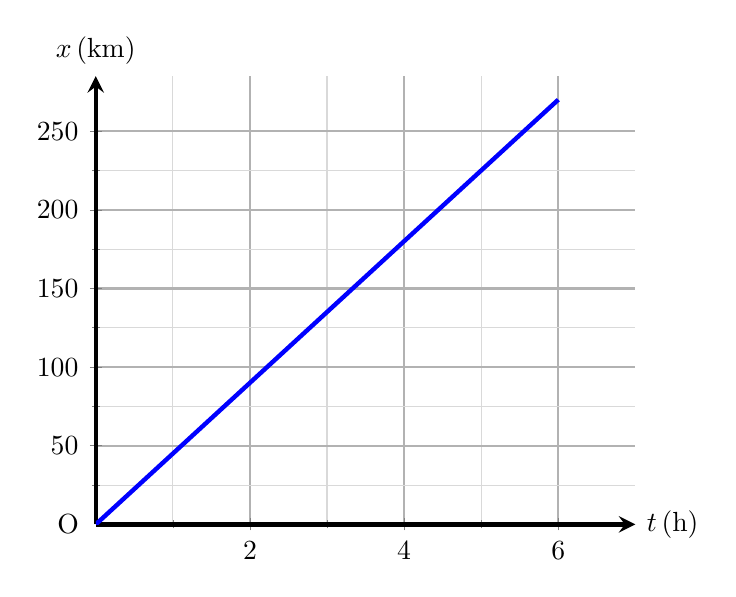
\begin{tikzpicture}  
			\begin{axis}[  ultra thick,
				xmin=0,  
				xmax=7,  
				xtick={0,2,...,6},
				ytick={0,50,...,250},
				minor x tick num=1,
				minor y tick num=1,
				ymin=0,  
				ymax=285, 
				samples=300,
				axis lines=center, 
				grid style={step=1, line width =0.4pt, color=gray!30!white},
				grid=both, %giới hạn ô lưới
				major grid style={line width=0.8pt,gray!60!white},
				xlabel=$\xsi{t}{\left(\si{\hour}\right)}$, 		ylabel=$\xsi{x}{\left(\si{\kilo\meter}\right)}$,
				every axis y label/.style={at=(current axis.above origin),anchor=south},  
				every axis x label/.style={at=(current axis.right of origin),anchor=west},  ] 
				\addplot [ultra thick, blue, smooth, domain=0:6] {45*x}; 
			\end{axis} 
		\node at (-0.35,0) {O}; 
		\end{tikzpicture}
		
	\end{center}
	\choice
	{\True $\SI{45}{\kilo\meter/\hour}$}
	{$\SI{43.75}{\kilo\meter/\hour}$}
	{$\SI{45.45}{\kilo\meter/\hour}$}
	{$\SI{50}{\kilo\meter/\hour}$}
	\loigiai{
Tại $t=\SI{5}{\hour}$ thì $x=\SI{225}{\kilo\meter}$:
$$\left|v\right|=\left|\dfrac{\Delta x}{\Delta t}\right|=\SI{45}{\kilo\meter/\hour}.$$	
}
\end{ex}


\Closesolutionfile{ans}
\section{Câu trắc nghiệm đúng/sai} 
\textit{Trong mỗi ý \textbf{a)}, \textbf{b)}, \textbf{c)}, \textbf{d)} ở câu bên dưới, thí sinh chọn đúng hoặc sai}
\setcounter{ex}{0}
\Opensolutionfile{ans}[ans/G10C1TF]
% ===================================================================
\begin{ex}
Một bạn học sinh dùng volt kế để đo hiệu điện thế hai đầu điện trở. Kết quả trong một lần đo được ghi nhận như hình bên dưới.
\begin{center}
	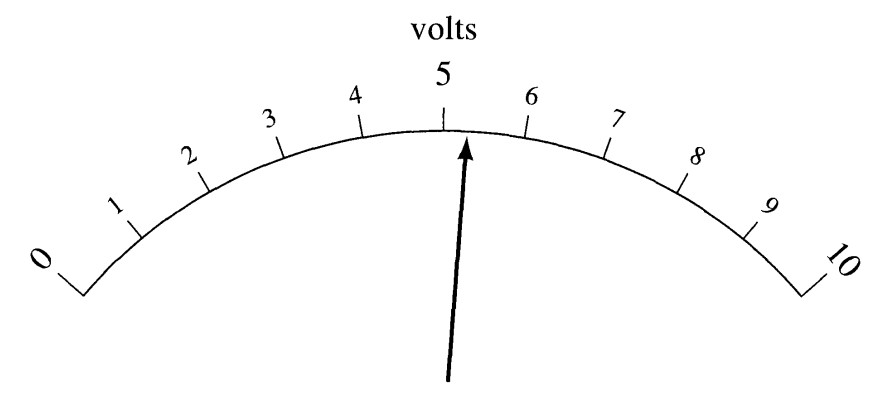
\includegraphics[width=0.6\linewidth]{figs/G10-CHUONG1-2}
\end{center}
	\choiceTF[t]
	{\True Độ chia nhỏ nhất của volt kế trên là $\SI{1}{\volt}$}
	{Kết quả lần đo trên hình nên được đọc là $\SI{5.25}{\volt}$}
	{Có thể hạn chế sai số hệ thống bằng cách thực hiện phép đo nhiều lần}
	{\True Kết quả đo có thể mắc sai số ngẫu nhiên do thao tác của người đo hoặc các yếu tố bên ngoài tác động}
	\loigiai{
\begin{itemchoice}
	\itemch Đúng.
	\itemch Sai. ĐCNN của volt kế là $\SI{1}{\volt}$ nên chỉ có thể đọc được giá trị $\SI{5}{\volt}$ hoặc $\SI{6}{\volt}$. Quan sát chủ quan thấy kim nằm gần vạch $\SI{5}{\volt}$ hơn.
	\itemch Sai. Sai số hệ thống được hạn chế bằng cách dùng dụng cụ có độ chia nhỏ nhất càng nhỏ và hiệu chỉnh dụng cụ đo về 0 trước khi đo.
	\itemch Đúng.
\end{itemchoice}	

}
\end{ex}

\Closesolutionfile{ans}
\section{Câu trắc nghiệm trả lời ngắn} \textit{Thí sinh trả lời từ câu 1 đến câu 6}
\setcounter{ex}{0}
\Opensolutionfile{ans}[ans/G10C1TL]
	% ===============================================================
\begin{ex}
Hố đen là một trong những đối tượng rất đặc biệt trong vũ trụ. Nguồn gốc ra đời của hố đen bắt nguồn từ sự suy sụp hấp dẫn của một vật thể khối lượng rất lớn vào một điểm kỳ dị và tạo ra quanh nó một vùng không - thời gian cong vô hạn, nơi mà không thứ gì có thể thoát ra từ đó, kể cả ánh sáng. 
\begin{center}
	\begin{tabular}{M{7.5cm}M{7.5cm}}
		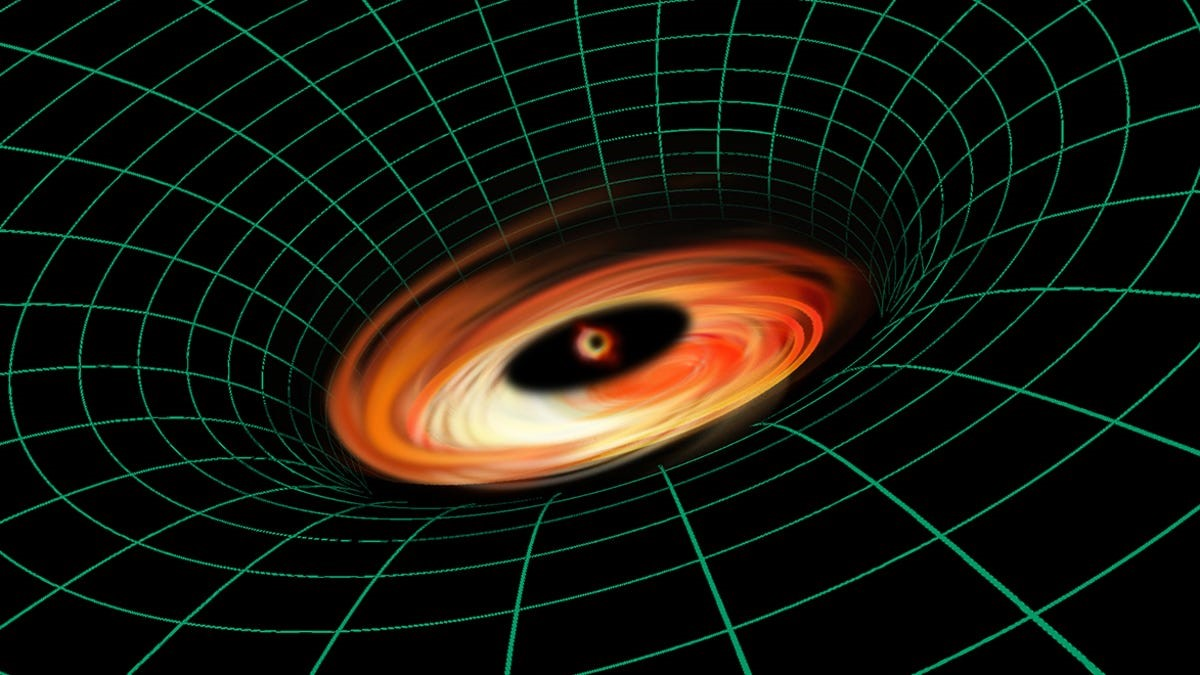
\includegraphics[width=0.7\linewidth]{figs/G10-CHUONG1-4}
		&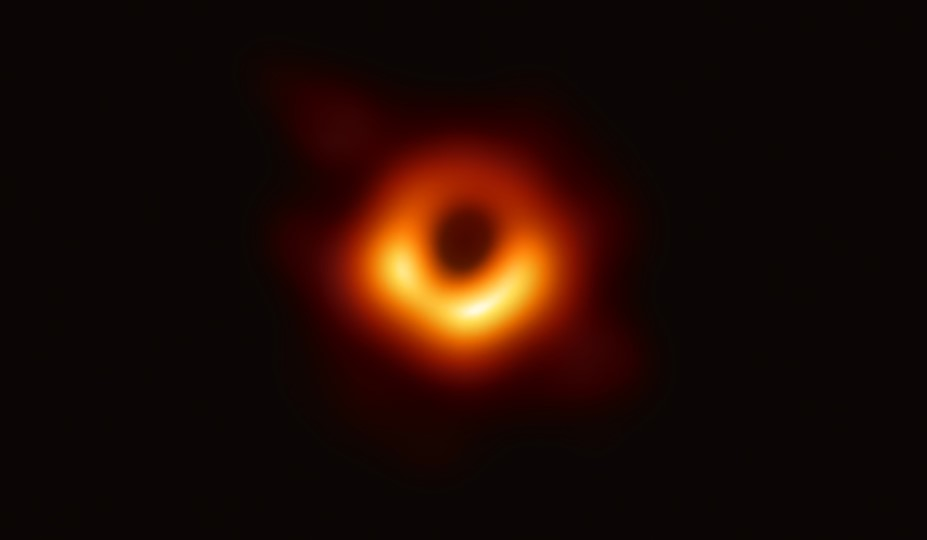
\includegraphics[width=0.7\linewidth]{figs/G10-CHUONG1-5}\\
		\textit{Minh hoạ hố đen làm cong không - thời gian}& \textit{Ảnh hố đen chụp bởi Kính viễn vọng chân trời sự kiện (EHT) và công bố năm 2019} 
	\end{tabular}
\end{center}
Theo nhà vật lí học người Đức Karl Schwarzschild, một vật thể có kích thước bằng với bán kính giới hạn (bán kính Schwarzschild) thì nó sẽ trở thành một hố đen. Bán kính  Schwarzschild được cho bởi công thức:
$$R_S=\dfrac{2GM}{c^2}$$
Trong đó:
\begin{itemize}
	\item $R_S$ là bán kính hấp dẫn Schwarzschild;
	\item $G$ là hằng số hấp dẫn;
	\item $M$ là khối lượng vật thể;
	\item $c$ là tốc độ ánh sáng trong chân không.
\end{itemize}
Trong công thức trên, hằng số hấp dẫn có thứ nguyên là $L^\alpha M^{-\beta}T^{-\gamma}$. Với $\alpha$, $\beta$, $\gamma$ là các số nguyên dương. Xác định giá trị của $\alpha\beta\gamma$.

	\shortans{312 }
	\loigiai{
		Ta có:
		$$G=\dfrac{1}{2}\dfrac{R_Sc^2}{M}.$$
		Phân tích thứ nguyên:
		$$\left[G\right]=\dfrac{\left[R_S\right]\times\left[c\right]^2}{\left[M\right]}=\dfrac{L\times\left(LT^{-1}\right)^2}{M}=L^3M^{-1}T^{-2}\Rightarrow \begin{cases}
			\alpha=3\\
			\beta=1\\
			\gamma=2
		\end{cases}.$$
	}
\end{ex}
	% ===============================================================
\begin{ex}
	Một nhóm học sinh đo được hiệu điện thế giữa hai đầu một điện trở là $U=\xsi{\left(10,0\pm0,3\right)}{\volt}$ và cường độ dòng điện qua điện trở là $I=\xsi{\left(1,3\pm0,2\right)}{\ampere}$. Tính sai số tương đối trong phép đo điện trở \textit{(Kết quả tính theo đơn vị $\si{\percent}$ và làm tròn đến 3 CSCN)}.\\
	Cho biết giá trị của điện trở được xác định bởi $R=\dfrac{U}{I}$.
	\shortans{18,4 }
	\loigiai{
		Giá trị điện trở:
		$$R=\dfrac{U}{I}.$$
		Sai số tương đối của phép đo:
		$$\delta R=\left(\dfrac{\Delta U}{\overline{U}}+\dfrac{\Delta I}{\overline{I}}\right)\cdot\SI{100}{\percent}\approx\SI{18.4}{\percent}.$$
	}
\end{ex}
\textit{Dữ kiện sau đây được dùng chung cho câu 3 đến câu 6}\\
Bạn An thực hiện thí nghiệm đo tốc độ chuyển động thẳng với dụng cụ và sơ đồ bố trí thí nghiệm như hình bên dưới.
Trong đó, hai cổng quang điện A và B được đặt cách nhau $\SI{30}{\centi\meter}$ và được nối với đồng hồ đo thời gian hiện số (1) được đặt ở chế độ đo với sai số dụng cụ $\SI{0.01}{\second}$. Độ chia nhỏ nhất của thước đo (5) là $\SI{0.5}{\centi\meter}$.
\begin{center}
	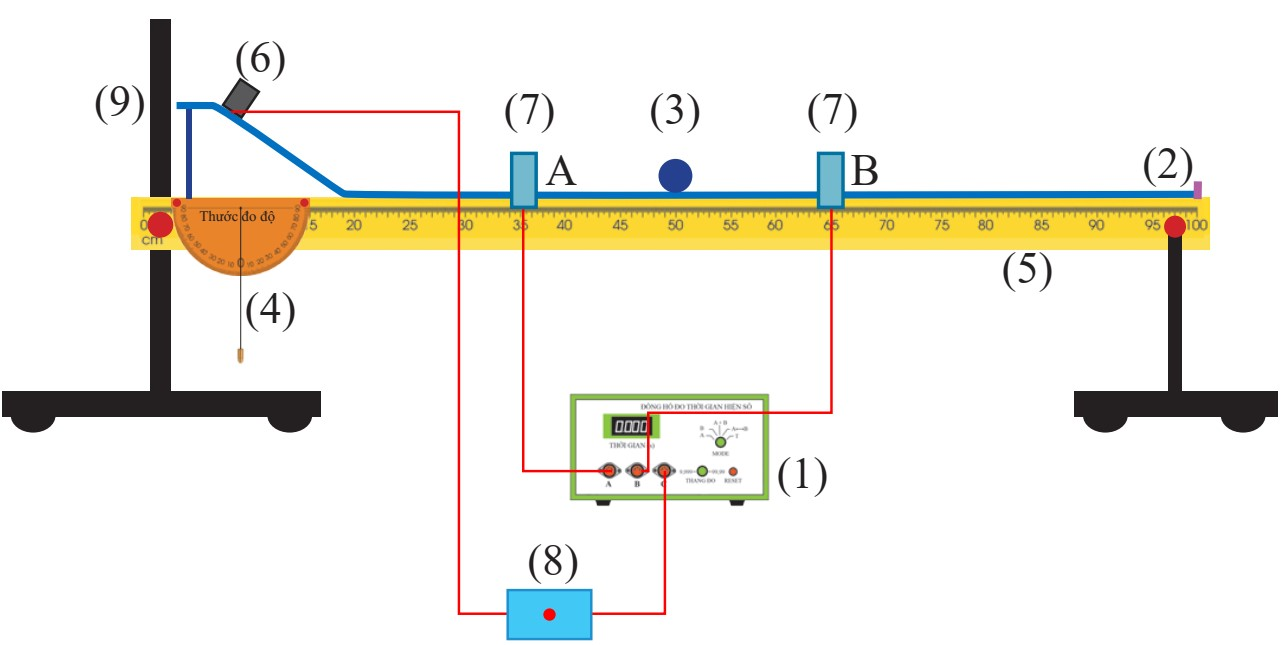
\includegraphics[width=0.75\linewidth]{../figs/G10-CHUONG1-3}
\end{center}
Bạn An thiết đặt đồng hồ đo thời gian hiện số ở chế độ A$\leftrightarrow$B để đo thời gian viên bi chuyển động kể từ khi chắn qua cổng quang A đến khi qua cổng quang B. Sau 5 lần đo, An ghi nhận được các giá trị thời gian chuyển động của viên bi như bảng bên dưới:
\begin{center}
	\begin{longtable}{|M{4cm}|M{2cm}|M{2cm}|M{2cm}|M{2cm}|M{2cm}|}
		\hline
		\thead{Lần đo}&1&2&3&4&5\\
		\hline
		\thead{Thời gian $\left(\si{\second}\right)$}& 4,75 & 4,68 & 4,73 & 4,68 & 4,70\\
		\hline
	\end{longtable}
\end{center}
\textit{* Lưu ý: Trong các phần tính toán bên dưới, các giá trị trung bình được lấy cùng bậc thập phân với giá trị đo.}
	% ===============================================================
\begin{ex}
Xác định thời gian chuyển động trung bình của viên bi \textit{(Kết quả tính theo đơn vị giây và làm tròn đến 3 CSCN)}.
	\shortans{4,71}
	\loigiai{
		Thời gian chuyển động trung bình của viên bi:
	$$\overline{t}=\dfrac{t_1+t_2+\dots+t_5}{5}=\SI{4.708}{\second}\approx\SI{4.71}{\second}.$$	
	}
\end{ex}
	% ===============================================================
\begin{ex}
Xác định sai số tương đối trong phép đo trên \textit{(Kết quả tính theo đơn vị $\si{\percent}$ và làm tròn đến 3 CSCN)}.
	\shortans{0,85}
	\loigiai{
		\begin{center}
			\begin{longtable}{|M{2cm}|M{4cm}|M{2cm}|}
				\hline
				\thead{Lần đo} & $\xsi{t}{\left(\second\right)}$ &$\xsi{\Delta t}{\left(\second\right)}$\\
				\hline
				1 & 4,75 &0,04 \\
				\hline
				2 & 4,68 & 0,03\\
				\hline
				3 & 4,73 & 0,02\\
				\hline
				4 & 4,68 & 0,03\\
				\hline
				5 & 4,70 & 0,01\\
				\hline
				\thead{TB}&4,71&0,03\\
				\hline
			\end{longtable}
		\end{center}
	Sai số tuyệt đối của phép đo thời gian:
	$$\Delta t=\overline{\Delta t}+\Delta t_{\text{dc}}=\SI{0.03}{\second}+\SI{0.01}{\second}=\SI{0.04}{\second}.$$
Sai số tương đối của phép đo thời gian:
$$\delta t=\dfrac{\Delta t}{\overline{t}}\cdot\SI{100}{\percent}=\dfrac{\SI{0.04}{\second}}{\SI{4.71}{\second}}\cdot\SI{100}{\percent}\approx\SI{0.85}{\percent}.$$}
\end{ex}
	% ===============================================================
\begin{ex}
	Xác định tốc độ trung bình của viên bi trong thí nghiệm trên \textit{(Kết quả tính theo đơn vị $\si{\centi\meter/\second}$ và làm tròn đến 3 CSCN)}.
	\shortans{6,37}
	\loigiai{
		$$\overline{v}=\dfrac{\overline{s}}{\overline{t}}=\dfrac{\SI{30}{\centi\meter}}{\SI{4.71}{\second}}\approx\SI{6.37}{\centi\meter/\second}.$$
	}
\end{ex}
	% ===============================================================
\begin{ex}
	Xác định sai số tuyệt đối trong phép đo tốc độ trung bình của viên bi \textit{(Kết quả tính theo đơn vị $\si{\centi\meter/\second}$ và làm tròn đến 3 CSCN)}.
	\shortans{0,11}
	\loigiai{
		ĐCNN của thước (5) là $\SI{0.5}{\centi\meter}$ nên sai số $\Delta s=\dfrac{\SI{0.5}{\centi\meter}}{2}=\SI{0.25}{\centi\meter}$.\\
		Sai số tuyệt đối trong phép đo tốc độ trung bình:
		$$\dfrac{\Delta v}{\overline{v}}=\dfrac{\Delta s}{\overline{s}}+\dfrac{\Delta t}{\overline{t}}\Rightarrow \Delta v=\left(\dfrac{\Delta s}{\overline{s}}+\dfrac{\Delta t}{\overline{t}}\right)\cdot\overline{v}=\left(\dfrac{\SI{0.25}{\centi\meter}}{\SI{30}{\centi\meter}}+\dfrac{\SI{0.04}{\second}}{\SI{4.71}{\second}}\right)\cdot\left(\SI{6.37}{\centi\meter/\second}\right)\approx\SI{0.11}{\centi\meter}.$$
	}
\end{ex}
\Closesolutionfile{ans}
\begin{center}
	\textbf{--- HẾT ---}
\end{center}

\end{document}